\hfill На правах рукописи

\vspace{\baselineskip}
\vspace{\baselineskip}
\vspace{\baselineskip}

\noindent\centerline{\bf{Никифоров Александр Александрович}}

\vspace{\baselineskip}
\vspace{\baselineskip}
\vspace{\baselineskip}

\noindent\centerline{ИДЕНТИФИКАЦИЯ И ОЦЕНКА ИНФОРМАЦИОННЫХ ПАРАМЕТРОВ}
\noindent\centerline{НАВИГАЦИОННЫХ СИСТЕМ С КОДОВЫМ РАЗДЕЛЕНИЕМ}

\vspace{\baselineskip}
\vspace{\baselineskip}
\vspace{\baselineskip}

\noindent\centerline{Специальность 05.13.01. – Системный анализ,}
\noindent\centerline{управление и обработка информации}

\vspace{\baselineskip}
\vspace{\baselineskip}
\vspace{\baselineskip}

\noindent\centerline{Автореферат} 
\noindent\centerline{диссертации на соискание ученой степени}
\noindent\centerline{кандидата технических наук}


\vfill
\noindent\centerline{Москва – 2014}

\pagenumbering{gobble}
\newpage
%%%%%%%%%%%%%%%%%%

\noindent\centerline{Работа выполнена в федеральном государственном бюджетном образовательном}
\noindent\centerline{учреждении высшего профессионального образования}
\noindent\centerline{«Московский Государственный Технический Университет имени Н.Э. Баумана»}
\vspace{\baselineskip}

\noindent\begin{tabular*}{\columnwidth}{@{\extracolsep{\stretch{1}}}*{6}{l l}@{}}
{\bf{Научный руководитель}} -	& 	Сидоркина Юлия Анатольевна, кандидат \\
       			&	технических наук, доцент кафедры автономных\\
			&	информационных и управляющих систем \\
			&	МГТУ им. Н.Э. Баумана\\
{\bf{Официальные оппоненты}}: 	& Первый оппонент \\
       			&	Черныш Александр Викторович, кандидат\\
       			&	технических наук, начальник отдела цифровой  \\
      			&	обработки сигналов, ЗАО «Телум» \\
{\bf{Научный консультант}} -	& Мельников Алексей Олегович, кандидат\\
       			&	технических наук, доцент кафедры управление и\\
			&	моделирование систем \\
{\bf{Ведущая организация:}}	&	Название
\end{tabular*}
\vspace{\baselineskip}

\noindent
Защита диссертации состоится XX сентября 2014 г. в XX ч. XX мин. на заседании диссертационного совета Д 212.141.02 при федеральном государственном бюджетном
образовательном учреждении высшего профессионального образования «Московский Государственный Технический Университет имени Н.Э. Баумана» по адресу: 105005, Москва,
Госпитальный пер., д.10., ауд.613м. www.bmstu.ru.

\noindent
С диссертацией можно ознакомиться в библиотеке МГТУ им. Н.Э. Баумана.
\noindent
Отзывы и замечания по автореферату в двух экземплярах, заверенные печатью, просьба высылать по вышеуказанному адресу на имя ученого секретаря диссертационного совета.
Автореферат разослан \_\_\_ июня 2014 г.

\vfill
\noindent
Ученый секретарь диссертационного совета, 
к.т.н., доц. 	Муратов И.В. 

\pagenumbering{gobble}
\newpage

% switch page on
\pagenumbering{arabic}

%\addcontentsline{toc}{section}{ВВЕДЕНИЕ}
{\center{\section*{ОБЩАЯ ХАРАКТЕРИСТИКА РАБОТЫ}}}

{\bf{Актуальность работы}}

Диссертационная работа Никифорова Александра Александровича посвящена проблеме оценки информационных параметров в системах с кодовым разделением каналов
(в англоязычной литературе CDMA - code division multiple access).
Технология CDMA получила широкое распространение в современных стандартах цифровой связи и продолжает активно развиваться. Она позволяет добиваться высокой
спектральной и энергетической эффективности, высокой помехозащищенности, позволяет эффективно бороться с многолучевым распространением радиоволн.
Перспективным применением технологии CDMA являются устройства управления и передачи информации в системах связи и навигации, таких как Skylink и Navstar GPS. 

Наряду с очевидными достоинствами, CDMA-системы обладают рядом существенных недостатков. К недостаткам можно отнести: на приемной стороне необходимо рассматривать
двумерную область неопределенности при отсутствии априорных данных для каждого источника сигнала, низкое разрешение при оценке информационных параметров сигнала при типовом подходе
к решению данной задачи.

Проблемам оценивания информационных параметров сигнала в системах передачи информации посвящены работы как отечественных так и зарубежных исследователей.
В России в данной области работают: В.И. Борисов, В.Б. Пестряков, В.И. Журавлев, М.И. Жодзишский,
Б.И. Шахтарин, Л.Е. Варакин, В.Е. Гантмахер.
Среди зарубежных исследователей в этой области необходимо отметить работы Дж. Спилкера, М.К. Саймона, Дж.К. Омура, Д.Дж. Торьери, Дж. Прокис, Дж. Цуя, Э. Каплана.
Используемые современными исследователями типовые алгоритмы имеют потенциал совершенствования как в вопросах увеличения точности оценок
информационных параметров сигнала, так и в вопросах уменьшения вычислительной сложности.
Помимо этого следует отметить что развитие современной элементной базы привело к появлению дешевых цифровых процессоров, оснащенных модулем для вычислений
с плавающей точкой, а также распространению программных приемников, работающих на аппаратном обеспечении общего назначения. Это делает возможным применение новых
подходов к обработке информационных сигналов систем с кодовым разделением каналов в реальном времени, вместо использовавшейся отложенной обработки данных и данная
тема является актуальной.

{\bf{Цель и задачи диссертации}}

Целью диссертационной работы является разработка и анализ алгоритмов оценки информационных параметров сигнала в системах с кодовым разделением каналов на основе
параметрического метода оценки частоты на фоне аддитивного белого гауссового шума и интерференционной помехи,
с возможностью реализации на современной элементной базе.

Для достижения поставленной цели в диссертации решаются следующие задачи:
\begin{enumerate}
	\item {С использованием методов параметрической идентификации автором разработка алгоритма оценки информационных параметров для одного источника сигнала
		в CDMA-системах на фоне аддитивного белого гауссового шума.}
	\item {Адаптация алгоритма повышения отношения сигнал/шум при оценке автокорреляционной функции гармонического сигнала для использования при обработке
		CDMA-сигнала в приемниках реального времени.}
	\item {Разработка комплексированного алгоритма оценки информационных параметров CDMA-сигнала на фоне аддитивного белого гауссового шума и
		интерференционной помехи, основанный на алгоритме Delay and Multiply Approach, алгоритме повышения сигнал/шум в оценке автокорреляционной функции 
		и авторегрессионной модели второго порядка.}
	\item {Сравнительный анализ разработанных алгоритмов с типовыми решениями в области оценки информационных параметров сигнала используемых в CDMA-системах.}
	\item {Полунатурное моделирование с использованием аппаратной платформы на реальных данных CDMA-системы Navstar GPS.}
\end{enumerate}

{\bf{Научная новизна результатов}}

\begin{enumerate}
	\item{На основе теории параметрической идентификации автором разработан алгоритм оценки информационных параметров сигнала в системах с кодовым разделением каналов.}
	\item{Предложен алгоритм компенсации окрашенного шума на основе итеративного вычисления автокорреляционной функции для
		получения несмещенной оценки частоты с использованием параметрического метода оценки спектра.}
	\item{Предложен способ эффективного итеративного вычисления автокорреляционной функции в базисе Фурье для использования в
		приемниках реального времени.}
	\item{Предложен способ комплексирования алгоритмов оценки фазы псевдослучайной последовательности (ПСП) Delay And Multiply Approach, алгоритма итеративной оценки АКФ и
		параметрического метода оценки спектра в задаче оценки параметров сигнала с расширенным спектром.}
\end{enumerate}

{\bf{Практическая ценность}}
\begin{enumerate}
	\item {Усовершенствован алгоритм повышения отношения сигнал/шум при оценке автокорреляционной функции. Оптимизация вычислительных затрат позволяет использовать
		данный алгоритм в приемниках реального времени.}
	\item {Получен алгоритм оценки информационных параметров CDMA-сигнала сна основе параметрического метода оценки спектра, усовершенствованного
		алгоритма повышения отношения сигнал/шум в оценке автокорреляционной функции и алгоритма Delay and Multiply Approach. Данный алгоритм
		позволяет свести перебор в двух областях неопределенности: фаза ПСП и промежуточная частота к перебору только в области фазы ПСП,
		что, в свою очередь, позволяет
		существенно снизить вычислительные затраты.}
	\item {Создан программно-аппаратный стенд для экспериментального исследования систем цифровой связи с использованием технологии CDMA,
		позволивший подтвердить схемотехническую реализуемость разработанных алгоритмов.}
\end{enumerate}

{\bf{Апробация результатов}}
Основные научные результаты докладывались и обсуждались на:
\begin{enumerate}
	\item 7-ой Всероссийской конференции "Радиолокация и радиосвязь" (Москва 2013)
	\item Международной конференции "Радиоэлектронные устройства и системы для инфокоммуникационных технологий - РЕС-2013" (Москва 2013)
	\item V Международной студенческой научно-практической конференции "Интеллектуальный потенциал XXI века: ступени познания" (Новосибириск 2011)
\end{enumerate}

{\bf{Внедрение результатов работы:}}
\begin{enumerate}
	\item Результаты диссертации использованы в НИОКР ЗАО «Теллум», что подтверждено актом о внедрении.
	\item Результаты диссертации использованы в учебном процессе на кафедрах автономных информационных и управляющих систем МГТУ им. Н.Э. Баумана,
		что подтверждено актом об использовании и управление и моделирование систем Московского Государственного Университета Приборостроения
		и Информатики, что подтверждено актом об использовании.
\end{enumerate}

{\bf{Объем и структура диссертации}}
Диссертация состоит из введения, четырех глав, заключения и списка литературы. Общий объем составляет XXX страниц, включающих XX страниц приложения, XX иллюстраций,
X таблицы и список литературы из XX наименований.

{\bf{Положения, выносимые на защиту}}
\begin{enumerate}
	\item {Алгоритм оценки информационных параметров CDMA-сигнала на фоне белого шума на основе АР-модели принимаемого сигнала.}
	\item {Алгоритм повышения отношения сигнал шум и подавления интерференционной помехи применительно к задаче оценки информационных параметров CDMA-сигнала.}
	\item {Алгоритм оценки информационных параметров CDMA-сигнала на фоне интерференционной помехи и шума на основе алгоритмов: Delay and Multiply Approach,
		усовершенствованного алгоритма итеративного вычисления автокорреляционной функции и АР-модели принимаемого сигнала.}
	\item {Результаты анализа точности, вычислительных затрат разработанных алгоритмов, а так же сравнительный анализ с типовым алгоритмом.}
\end{enumerate}

{\bf{Публикации по теме диссертации}}
Основные результаты получены Никифоровым А.А. самостоятельно и изложены в 5 научных работах, в том числе 4 статьи в журналах, рекомендованных ВАК и
3 докладах на международных конференциях.

%%%%

%\paragraph{Методы исследований.} Задачи исследования решаются при помощи методов теории сигналов, теории автоматического управления,
%методов параметрического спектрального анализа, методов математического и имитационного моделирования.
%
%\paragraph{Достоверность научных положений, результатов и выводов.}
%Достоверность выносимых на защиту положений подтверждена имитационным моделированием, полунатурным экспериментом и согласуется
%с известными результатами.


%paragraph{Личный вклад автора.}
%В основу диссертации легли результаты исследований, выполненных лично автором на кафедре «Управление и моделирование систем» Московского Государственного
%Университета Приборостроения и Информатики. Личный вклад автора состоял также в непосредственном участии в получении исходных данных, в апробации результатов исследования,
%в подготовке основных публикаций по выполненной работе.

{\center\section*{КРАТКОЕ СОДЕРЖАНИЕ РАБОТЫ}}

% Include text from phd
\addcontentsline{toc}{section}{ВВЕДЕНИЕ}
\section*{ВВЕДЕНИЕ}

Большое количество современных систем являются беспроводными. Простота развертывания, мобильность, относительно низкая
стоимость - вот основные преимущества беспроводных систем. Количество мобильных устройств (телефоны, планшетные компьютеры
и т.д.) с каждым годом стремительно растет, только мобильных телефонов в 2011 году было 5.6 миллиарда и покрывало 79.86\%
\cite{wiki_mobilenum} населения земли. Технологии беспроводной связи глубоко проникли во все сферы жизни общества:
обеспечение безопасности с помощью RFID датчиков, предоставление доступа в интернет по технологиями 3G, WiFi, 
сотовая связь по различным технологиям (GSM, CDMA, DAMPS). Некоторые из этих систем строятся на основе методики
расширения спектра, которая отвечает современным требованиям по мощности сигнала, а так же по безопасности передаваемых
данных. В основе таких систем лежат шумоподобные (широкополосные) сигналы - ШПС. Вместе с тем растут требования к таким
системам. Применение ШПС ставит ряд специфических задач по обработке информации, обусловленных особенностями ШПС.
Свойства характерные для ШПС, выгодно отличают данный класс систем от класса узкополосных систем, но с другой стороны
оборачивается усложнением методов обработки ШПС.

Внедрение новых технологий требует увеличение полосы частот. Разнообразие технологий беспроводной передачи данных среди
гражданских и военных систем ведет к перегрузке каналов связи и все более высоким требованиям к скорости передачи
данных. С учётом данных требований применение систем передачи информации с ШПС становится все более востребованным.

Принимая во внимание географические размеры России и стратегическую важность обладания собственными системами спутникового
позиционирования, правительство Российский Федерации уделяет особое внимание разработке собственной системы
глобального спутникового позиционирования ГЛОНАСС. Обладание собственными технологиями системы спутниковой навигации (СНС), государство может обезопасить
себя в случае военных конфликтов от ограничения применения американской системы СНС Navstar GPS в зоне конфликта.

Разработка систем, позволяющих работать с несколькими различными СНС, позволит повысить точность определения координат
в сложных условиях города. Сложность детектирования сигнала и определения координат обусловлена наличием плотной
застройки многоэтажными зданиями. В городских условиях задача подавления интерференционной помехи становится особенно
актуальной. Спектр интерференционной помехи не является белым, а фильтрация и компенсация цветного шума
требует разработки специальных алгоритмов.

Новые цифровые процессоры позволяют применять подходы, которые еще 10-15 лет назад были бесперспективными.
В данной работе развиваются подходы на основе построения параметрической модели ШПС. Невозможность использования
методов требующих вычислений с высокой точностью в приемниках реального времени
10-15 лет назад была обусловлена слабой производительностью процессоров и микроконтроллеров, а так же существенной
стоимостью процессоров с модулем для операций с числами с плавающей точкой. Современное развитие цифровых технологий делает 
возможным применение параметрических методов оценки спектра взамен традиционного подхода основанного на непараметрического
анализа спектра.

Основа теории систем связи с ШПС была заложена в работах В.А. Котельникова и К. Шеннона.
России в этой области занимались В.И. Борисов, В.Б. Пестряков, В.И. Журавлев, М.И. Жодзишский, Б.И. Шахтарин, Л.Е.  Варакин, В.Е. Гантмахер и др.

Изначально методы расширенного спектра применялись при разработке военных систем управления и связи \cite{sklyar}.
К концу второй мировой войны расширение спектра применялось в радиолокации для борьбы с преднамеренными помехами, а
в последствии развитие данной технологии объяснялось желанием создать помехоустойчивые системы связи.
В конце 40-х-начале 50-х годов прошлого века Мортимер Рогофф, сотрудник Международной Телефонной и Телеграфной Корпорации (США) (ITT),
провёл эксперимент по передаче информации при помощи псевдошумового сигнала \cite{sklyar}, среди отечественных ученых
в середине 30-х годов прошлого века работу об основах кодового разделения каналов написал Д.В. Агеев.
Первые разработки таких систем относились к военным отраслям. Данный факт объясняется рядом особенностей, которыми обладают
сигналы с расширенным спектром, в числе которых — сложность перехвата заложенной в них информации,
высокая помехоустойчивость, а также трудность обнаружения факта работы передатчика. В процессе исследований расширенному спектру
нашлось и другое применение - снижение плотности энергии, высокоточная локация, использование при множественном доступе
\cite{sklyar}

Системы связи с широкополосными сигналами занимают особое место. Их особенные свойства выделяют данный класс из других систем
связи. Высокая помехозащищенность при действии сильной помехи, кодовое разделение большого количества абонентов, прием
информации с высокой достоверностью - отличительные особенности широкополосных система. Эти черты были известно, но
уровень элементной базы и низкий уровень помех не позволяли получить развития системам данного класса. Однако развитие
элементной привело к широкому распространению данного вида сигналов. В настоящее они применяются в системах спутниковой навигации,
системах сотовой связи и др \cite{varakin-book}.

Отношение сигнал/шум (ОСШ) на входе приемника может быть очень низким. Для обеспечения высокой помехозащищенности 
в таких случаях используются ШПС с большими и сверхбольшими базами.

К созданию сложных широкополосных сигналов (СШС) привело решение ряда проблем при развитии систем передачи данных.
Первая проблема встала при разработке новых радиолокационных система. Для дальнейшего развития требовалось
решить несколько противоречий: требование высокой разрешающей способности по дальности и дальностью обнаружения
целей в импульсных РЛС, требование точного измерения скорости и высокое разрешение по дальности, требование
увеличить дальность при ограничении пиковой мощности \cite{gantmaher-book}. Решение данных задач было предложено
Ф. Вудвардом. Им было показано, что дополнительным параметром является форма сигнала. Длительность сигнала
может быть больше - настолько больше, насколько это необходимо для обеспечения энергетических требований, а требование
разрешения по дальности и точности измерений определяются шириной полосы сигнала. Данные требования обеспечивается
путем сжатия импульса на стороне приемника. Вудворд сформулировал принципы: произведение эффективной полосы частот
радиосигнала на его длительность должен быть существенно больше единиц ${FT>>1}$, внутренняя структура сигнала
должна быть такой, чтобы обеспечить возможность приемнику сжатие распределенного во времени сигнала в короткий импульс,
соответствующий полосе ${F}$ \cite{gantmaher-book}.

В \cite{gantmaher-book} показана связь пропускной способности канала с понятием ШПС. При ${R_e<<1}$ можно записать:
\begin{center}
\begin{equation}
	\label{eq:shennon_cdma}
	FT = \frac{1}{\log(1+R_e)},
\end{equation}
\end{center}
где ${R_e}$ - ОСШ, ${F}$ - эффективная полоса частот, ${T}$ - длительность.

Стоить отметить, что при ${R_e<<1}$, левая часть выражения \ref{eq:shennon_cdma} стремится к бесконечности, а значит
ШПС позволяет обеспечить теоретически неограниченную достоверность передачи информации. Второе важное свойство
ШПС, следующее из \ref{eq:shennon_cdma} - способность работать "под шумами". Что обеспечивает скрытность
передачи информации, а с другой высокую степень уплотнения каналов связи и, как следствие, решение современных проблем
с перегруженностью каналов связи.

В данной работе будет рассматриваться ШПС модулированный ПСП на основе двоичной рекуррентной последовательности.
Для выделения данных из потока необходимо иметь точно синхронизированную копию ПСП, которая была использована
при модулировании сигнала на передающей стороне. Для достижения синхронизма на стороне приемника необходимо
устранить неопределенность в двух областях: неопределенность по частоте и неопределенность по фазе (задержке) ПСП.
Неопределенность по фазе ПСП обусловлена неопределенностью в расстоянии между передатчиком и приемником. Неопределенность
по частоте обусловлена в первую очередь допплеровским эффектом, а так же нестабильностью опорных генераторов в
передатчике и приемнике. После устранения неопределенности по частоте для достижения точной синхронизации
начинается процесс слежения за частотой. Неопределенность по фазе ПСП устранить, не используя полный перебор,
невозможно в силу корреляционных свойств ПСП. Таким образом можно заключить, что задача быстрого и эффективного
поиска и оценки параметров ШПС является актуальной.

В данной работе рассматривается подход программного приемника (Software Defined Receiver - SDR)
\cite{akos-book, grayver-book, pany-book} для оценки параметров ШПС. Как уже было отражено выше, ШПС применяется во
многих системах. В данной работе для полунатурного эксперимента будет рассматриваться сигнал СНС Navstar GPS. Данная система передачи 
информации использует ПСП Голда \cite{gold-ieee} для модулирования сигнала.

Традиционные подходы к реализации приемника СНС Navstar GPS отражены в \cite{akos-book, tsui}. 

Популярность и распространенность данной системы стимулирует исследования в области детектирования
и оценки частоты ШПС сигналов.

Существуют исследования в области применения теории хаоса - детектирование и оценка
частоты ШПС с применением осциллятора Дуффинга \cite{chaos_cambridge, chaos_chen, chaos_huang, chaos_wang}. Преимуществом
данного подхода является то, что свойства осциллятора позволяют детектировать сигналы с экстремально низким ОСШ. В то же
время, на данный момент никто не предложил цифровое представление осциллятора Дуффинга, а это затрудняет использование данного подхода
в реальных приемниках. Таким образом данное направление является в настоящее время больше теоретическим, чем практическим.

В работах \cite{hos_petropulu, hos_zhao} предложено использовать статистики высоких порядков для подавления шума и детектирование
сигналов с низким уровнем ОСШ.

Более традиционные подходы для детектирования и оценки параметров ШПС сигналов с низким уровнем ОСШ рассмотрены в монографии \cite{ziedan-book}.
В данной монографии рассматриваются как методы детектирования и оценки параметров ШПС, основанные на когерентном накоплении, так и эффективные
системы слежения за частотой и фазой ПСП.

{\bf{Добавить ЦЕЛИ И ЗАДАЧИ}}

%%%%%%
\paragraph{Постановка задачи оценки параметров сигнала с расширенным спектром.}
В данной работе рассматриваются задачи повышения рабочих характеристик приемников ШПС, поэтому целесообразно отразить основные модули этой системы 
на примере СНС Navstar GPS - рисунок \ref{pic:sec1_gnss_system}.
\begin{figure}[H]
\center\scalebox{1}{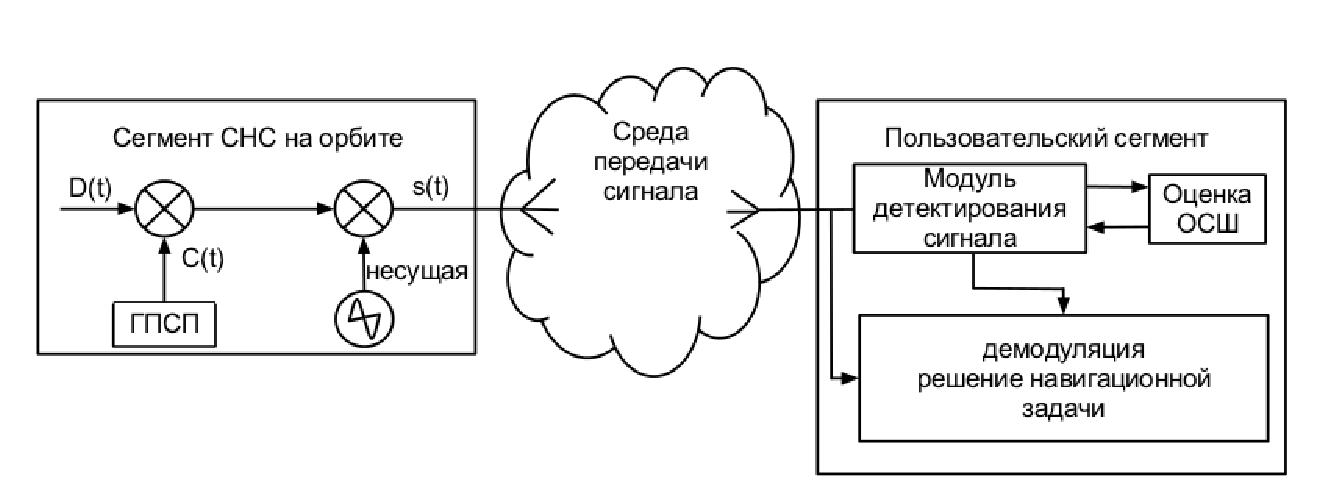
\includegraphics[width=1\linewidth]{sec1gnss_system.eps}}
\caption{структутраная схема СНС GPS}
\label{pic:sec1_gnss_system}
\end{figure}

В систему СНС Navstar GPS входят космический сегмент, наземный сегмент (на рисунке \ref{pic:sec1_gnss_system} не
отражен), а так же пользовательский сегмент. В космический сегмент входит спутниковая группировка, в 
наземный - станции управления, в пользовательский - все устройства принимающие сигнал от СНС GPS.

\paragraph{Модель сигнала и помех.}
В системе СНС Navstar GPS применяется ШПС.
Система передачи информации считается системой с расширенным спектром в следующих случаях \cite{sklyar}:
\begin{enumerate}
	\item Используемая полоса значительно шире минимальной, необходимой для передачи данных.
	\item Расширение спектра производится с помощью так называемого расширяющего сигнала (ПСП),
		который не зависит от передаваемой информации.
	\item Восстановление исходных данных ("сужение спектра") осуществляется путем сопоставления полученного
		сигнала и синхронизированной копии расширяющего сигнала (ПСП)
\end{enumerate}

Так же подобные сигналы называют:
\textquotedblleftсложными\textquotedblright,
\textquotedblleftшумоподобными\textquotedblright,
\textquotedblleftпсевдослучайными\textquotedblright,
\textquotedblleftсложными-дискретными\textquotedblright,
\textquotedblleftдискретно-кодированными\textquotedblright,
\textquotedblleftортогональными (квазиортогональными)\textquotedblright,
\textquotedblleftоптимальными дискретными\textquotedblright
\cite{gantmaher-book}.

Каждое название ставит акцент на определенной характеристике сигнала. В данной работе я буду оперировать термином
широкополосный сигнал - ШПС. ШПС можно определить как \cite{gantmaher-book, varakin-book}:
\begin{center}
\begin{equation}
	\label{eq:ss_signal}
	1 << FT = B,
\end{equation}
\end{center}
где: ${B}$ - база сигнала, ${F}$ - эффективная ширина спектра, а ${T}$ - длительность.
Неточность этого определения рассмотрена в \cite{gantmaher-book}, так же там даны ссылки на другие источники
разделяющие критику данного определения. Для данной работы критика, рассмотренная в приведенных источниках,
принципиального значения не имеет.

%%%%%%
\paragraph{Классическая постановка задачи оценки параметра.}
Из литературы по теории автоматических систем, например \cite{pugachev} (глава 10.1), известна классическая постановка
задачи задачи теории оптимальных систем. "На практике часто приходится решать задачу проектирования системы, когда
требуется определить характеристики системы таким образом, чтобы она имела наибольшую точность при данных условиях.
Систему обеспечивающую наибольшую возможную точность с какой-нибудь определенной точки зрения среди всех систем
заданного класса, обычно называют оптимальной" \cite{pugachev}.

В одной из постановок данной задачи \cite{pugachev} (глава 10.1), система считается полностью неизвестной
и требуется определить ее оператор так, чтобы она была оптимальной с точки зрения принятого критерия качества. Эта
задача сводится к определению с наибольшей возможной точностью некоторых параметров, от которых зависит принимаемый
сигнал. Но при этом важно учитывать не только точность, но и другие факторы, так как проектируемая система должна
удовлетворять многим, часто противоречивым требованиям. В виду приведенных факторов, обычно представляет собой
ряд компромиссных решений, удовлетворяющих всем предъявляемым к системе требованиям.

Точность автоматической системы обычно характеризуется математическим ожиданием и дисперсией ее ошибки.
Математическое ожидание представляет собой систематическую ошибку системы в данных условиях, а дисперсия
характеризует уровень случайных ошибок \cite{pugachev} (глава 10.2). Так как в различных условиях работы
системы, которые встречаются случайно систематическая ошибка тоже является случайной, за критерий качества
системы при ее проектировании обычно принимают второй начальный момент ошибки - математическое ожидание
квадрата ошибки:
\begin{center}
\begin{equation}
	\label{eq:stat_err_prob}
	\eta = M[e^2(t)]
\end{equation}
\end{center}
Положительный квадратный корень из этой величины называют средней квадратичной ошибкой системы. Таким образом,
оптимальной системой обычно считают такую систему, которая имеет минимальную среднюю квадратичную ошибку.

Критерий минимума средней квадратичной ошибки является простейшим с математической точки зрения и обычно приводит
к наиболее простым методам определения оптимальных систем. Однако далеко не во всех задачах он может служить мерой
качества системы. Поэтому нельзя ограничиваться методами нахождения оптимальных систем по критерию минимума средней
квадратичной ошибки.

В случаях, когда необходимо проектировать следящую систему, приходится учитывать возможность срыва слежения,
который заключается в том что система перестает работать, если ее ошибка превосходит по абсолютной величине некоторый
уровень. При проектировании таких систем целесообразно принять за критерий качества вероятность срыва слежения. При
этом оптимальной считается такая система, которая обеспечивает минимум вероятности срыва слежения. Если срыв слежения
происходит в случае, когда абсолютная величина ошибки превосходит уровень $a$, то критерий минимума вероятности ошибки
слежения можно представить \cite{pugachev} (глава 10.2):
\begin{center}
\begin{equation}
	\label{eq:prob_lost_signal}
	p = P(e(t) > a) = min
\end{equation}
\end{center}

%%%%%%
\paragraph{Введение обозначений.}
В диссертации рассматривается сигнал с расширенным спектром полученный методом "прямой последовательности".
Данный метод заключается в том, что гармоническая несущая сигнала модулируется высокоскоростным (широкополосным)
расширяющим сигналом (ПСП). 

Несущее колебание с частотой ${\omega_0}$  модулируется данными ${d(t)}$ , а также высокоскоростной ПСП ${g(t)}$, полученной методом "прямой последовательности".
СПИ Navstar GPS осуществляется двоичная фазовая модуляция (ДФМ или 2-ФМ), а значит ${d(t)}$  и ${g(t)}$  - потоки антиподных импульсов \{-1, 1\}.
Таким образом сигнал на выходе модулятора может быть представлен \cite{shahtarin_sync}:
\begin{equation}
	\label{eq:cdma_eq}
	s(t)=Ad(t)g(t)\cos{(\omega_{0}t)},
\end{equation}
где ${d(t)}$- информационный бит, а ${g(t)}$ - ПСП представляет собой фазовый сдвиг  ${0, \pi}$.

В реальных СПИ сигнал на приемник поступает одновременно от нескольких источников, присутствует неопределенность по частоте, а также аддитивный белый шум (АБГШ).
В приемнике после оцифровки сигнала получаем смесь:
\begin{equation}
	\label{eq:cdma_strip_eq}
	x(m)=\sum_{k=1}^{N}\left( A_k g(m + \tau_k)\exp{\left[j \left( \tilde{\omega}_{k}m + \phi_k(m)\right)\right]} \right) + n(m),
\end{equation}
где  ${k}$ - относительный номер источника сигнала, ${N}$ - количество доступных источников сигнала, модулированных ПСП одного семейства,
${m}$ - индекс соответствующий времени, ${\tilde{\omega}_{k}}$  – относительная частота, соответствующая ${\omega_0}$,
${\tau_k}$ - задержка модулирующей ПСП в точке приема, ${\phi_k(m)}$ - случайная начальная фаза, ${n(m)}$ - аддитивный белый гауссов шум (АБГШ). 

Следует отметить, что при оценке фазы сигнала с номером ${k}$  интерференцией являются сигналы:    .
\begin{equation}
	%\label{eq:cdma_interference}
	\{n \ne k, n \in [1,N]\}
\end{equation}

%%%%%%
\paragraph{Алгоритмы оценки параметров широкополосного сигнала сигнала.}
Алгоритм реализующий метод максимального правдоподобия - последовательный коррелятор. Данный подход реализуется в аппаратных приемниках.
Аппаратный приемник позволяет реализовать параллельно несколько последовательных корреляторов и вести оценку параметров
СПИ с ШПС параллельно.

Данный алгоритм в некоторых источниках так же называется согласованным фильтром. В \cite{sklyar} рассмотрены нюансы этих двух понятий.
В данной работе используется понятие последовательный коррелятор. Работа коррелятора описывается математической операцией
корреляции \ref{eq:serial_corr}. Сигнал коррелируется с локальной копией и на выходе коррелятора получается значение, отражающее
степень совпадения сигналов. Не трудно представить, что сигнал с хорошими корреляционными свойствами должен обладать высоким значением
корреляции когда сигналы синхронизированы и минимальным значением в любом другом случае (фаза ПСП не выровнена - отсутствие сигнала).
\begin{equation}
	\label{eq:serial_corr}
	y(n)=\sum\limits_{m=0}^{N-1}{x(m)h(n+m)},
\end{equation}
где ${x(m)}$ - принятая смесь, а ${h(n)}$ не импульсная характеристика системы, а локальная копия сигнала.

%%%%%%%%
% DFT

Вычисление циклической свертки через дискретное преобразование Фурье (ДПФ) - достаточно популярный метод
в программных приемниках, так как позволяет существенно уменьшить количество операций при вычислении. Но, как показано
в \cite{tsui, oppenheim}, можно достаточно просто перейти от свертки к циклической корреляции. Так как этот метод является самым
популярным в программных приемниках стоит его представить.
Свертка может быть представлена как:
\begin{equation}
	\label{eq:fft_conv}
	y(n)=\sum\limits_{m=0}^{N-1}{x(m)h(n-m)}
\end{equation}

Стоит отметить, что в \ref{eq:fft_conv} сдвиг во времени является циклическим, поскольку дискретные операции являются циклическими.
Возьмем ДПФ от \ref{eq:fft_conv}
\begin{center}
\begin{eqnarray}
	\label{eq:fft_conv_fft}
	Y(k) & = & \sum\limits_{n=0}^{N-1}\sum\limits_{m=0}^{N-1}{x(m)h(n-m)e^{(-j2\pi{kn})/N}}=\nonumber \\
	& = & \sum\limits_{m=0}^{N-1}{x(m)}[\sum\limits_{n=0}^{N-1}h(n-m)e^{(-j2\pi{(n-m)}k)/N}]e^{(-j2\pi{m}k)/N}=\\
	& = & H(k)\sum\limits_{m=0}^{N-1}e^{(-j2\pi{m}k)/N} = X(k)H(k)\nonumber 
\end{eqnarray}
\end{center}
Из уравнения \ref{eq:fft_conv_fft} легко видеть, что это не линейная свертка. В линейной свертке для входного сигнала размером в ${N}$ точек,
результат будет из ${2N-1}$ точек. А в уравнении выше, результатом является всего ${N}$ точек.
Это проявление циклической природы ДПФ.

Алгоритм оценки не использует свертку, он использует корреляцию, которая отличается от свертки. Корреляция
между $x(n)$ и $h(n)$ записывается выражением \ref{eq:serial_corr}:
Единственным отличаем между \ref{eq:serial_corr} и \ref{eq:fft_conv} является знак перед $m$ в ${h(n+m)}$.
В случае оценки параметра ШПС, $h(n)$ является локальной копией сигнала, а не импульсной характеристикой.
Произведем ДПФ над $z(n)$:
\begin{center}
\begin{eqnarray}
	\label{eq:fft_corr_fft}
	Z(k) & = & \sum\limits_{n=0}^{N-1}\sum\limits_{m=0}^{N-1}{x(m)h(n+m)e^{(-j2\pi{kn})/N}}=\nonumber \\
	& = & \sum\limits_{m=0}^{N-1}{x(m)}[\sum\limits_{n=0}^{N-1}h(n+m)e^{(-j2\pi{(n+m)}k)/N}]e^{(j2\pi{m}k)/N}=\\
	& = & H(k)\sum\limits_{m=0}^{N-1}e^{(j2\pi{m}k)/N} = X(k)H^{-1}(k)\nonumber 
\end{eqnarray}
\end{center}
где ${X^{-1}(k)}$ - обратное ДПФ. Уравнение \ref{eq:fft_corr_fft} можно записать как:

\begin{equation}
	\label{eq:fft_corr_fft_rev}
	Y(k) = \sum\limits_{n=0}^{N-1}\sum\limits_{m=0}^{N-1}{x(n+m)h(m)e^{(-j2\pi{kn})/N}}=X^{-1}(k)H(k)
\end{equation}

Если сигнал $x(n)$ действительный, то $x(n) = x^*(n)$, где ${^*}$ - операция комплексного сопряжения. Используя данное соотношение,
значение $Z(k)$ может быть записано:
\begin{equation}
	\label{eq:fft_magnitude}
	|Z(k)|=|H^*(k)X(k)|=|H(k)X(k)^*|
\end{equation}
Данное соотношение может быть использовано для нахождения значения циклической корреляции между входным сигналом и 
локальной копией.

%%%%%%%%
% Chaos 
Оценка параметров СПИ с ШПС (в частности сигналов системы Navstar GPS) с помощью осциллятора Дуффинга
достаточно новое направление в исследованиях по данной тематике. В данной области опубликовано несколько работ, в частности \cite{chaos_chen, chaos_cambridge, chaos_huang, chaos_song}.
Так же является интересной более ранняя статья не рассматривающая GPS \cite{chaos_wang}.
Осциллятор Дуффинга с гармоническим внешним воздействием может быть описан уравнением:
\begin{center}
\begin{equation}
	\label{eq:duffing}
	mx'' + cx' + k_{1}x + k_{2}x^3 = F_{0}\cos(\omega{t}),
\end{equation}
\end{center}
где $m$ - масса, $c$ - коэффициент диссипации, $x$ - состояние осциллятора, $k_1$ и $k_2$ - линейный и нелинейный коэффициенты соответственно,
$F_{0}\cos(\omega{t})$ - внешнее воздействие.

Подробно уравнение \ref{eq:duffing} рассмотрено в \cite{chaos_neimark_landa}.
Для использования осциллятора Дуффинга с целью оценки параметров ШПС была предложена усовершенствованная форма \cite{chaos_song, chaos_chen}:
\begin{center}
\begin{equation}
	\label{eq:duffing_gps}
	x'' +cx' - x^3 + x^5 = \gamma\cos(\omega{t}) + (\gamma_{x}\cos(\omega_{x}) + n(t))
\end{equation}
\end{center}

Перепишем динамическую систему \ref{eq:duffing_gps} в виде:
\begin{center}
\begin{equation}
	\label{eq:duffing_gps_2}
	\left\{
	\begin{aligned}
		y(t) & = x'(t) \\
		y'(t) & =  -cx' + x^3 - x^5 + \gamma\cos(\omega{t}) + (\gamma_{x}\cos(\omega_{x}) + n(t)),
	\end{aligned}
	\right.
\end{equation}
\end{center}
где ${n(t)}$ - АБГШ.

Пример фазового портрета при ${\omega=\omega_{x}}$ изображен на рисунке \ref{pic:duffing_sync},
фазовый портрет хаоса расположен на рисунках \ref{pic:duffing_chaos1}, \ref{pic:duffing_chaos2}
\begin{figure}[H]
	\center\scalebox{0.5}{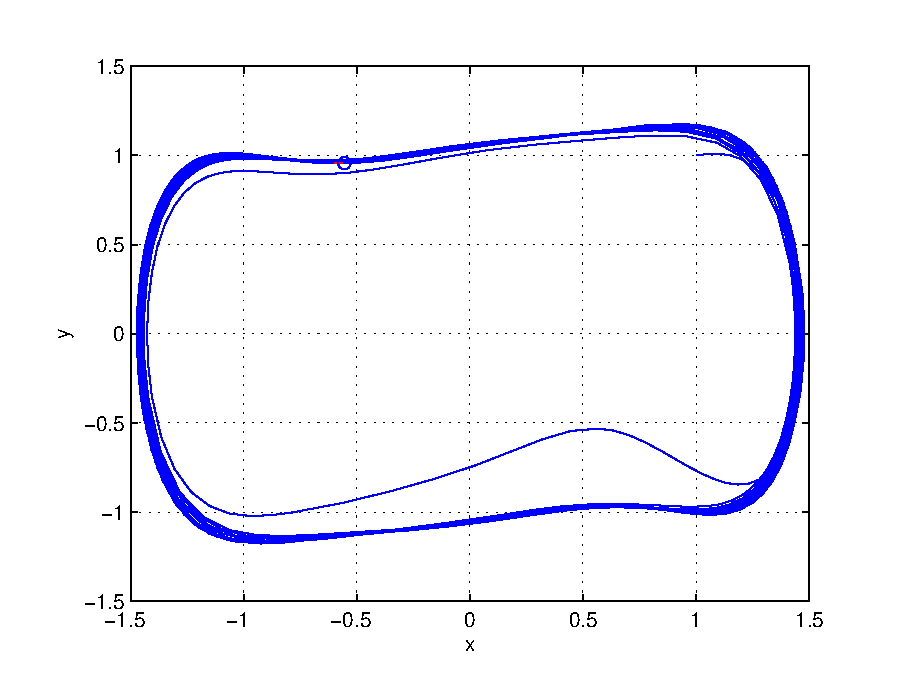
\includegraphics[width=1\linewidth]{duffing_sync.eps}}
	\caption{Фазовый портрет при ${\omega =\omega_{x}}$}
	\label{pic:duffing_sync}
\end{figure}
\begin{figure}[H]
	\center\scalebox{0.5}{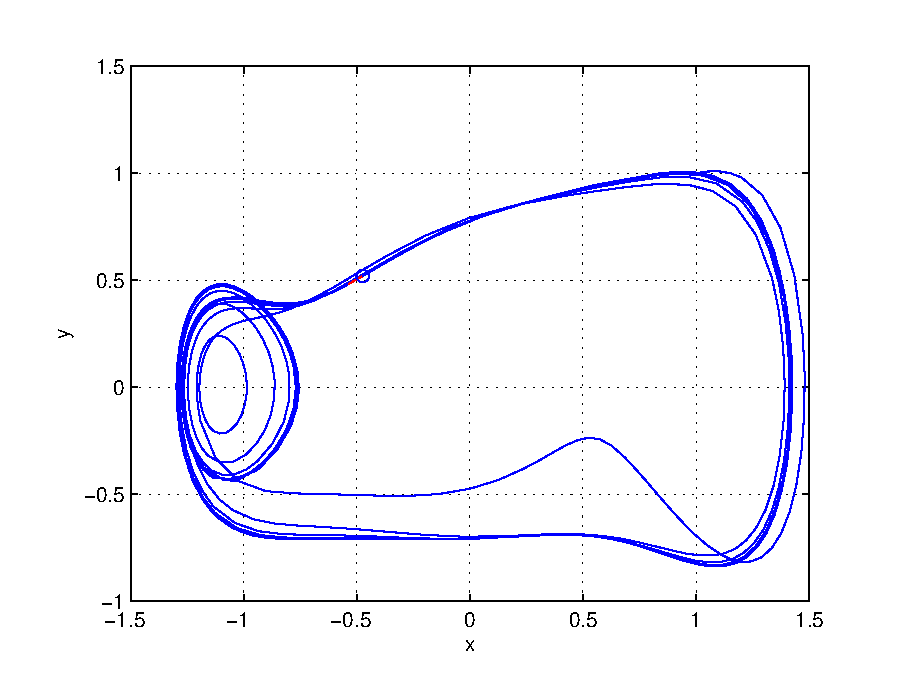
\includegraphics[width=1\linewidth]{duffing_chaos1.eps}}
	\caption{Фазовый портрет при ${\omega < \omega_{x}}$}
	\label{pic:duffing_chaos1}
\end{figure}
\begin{figure}[H]
	\center\scalebox{0.5}{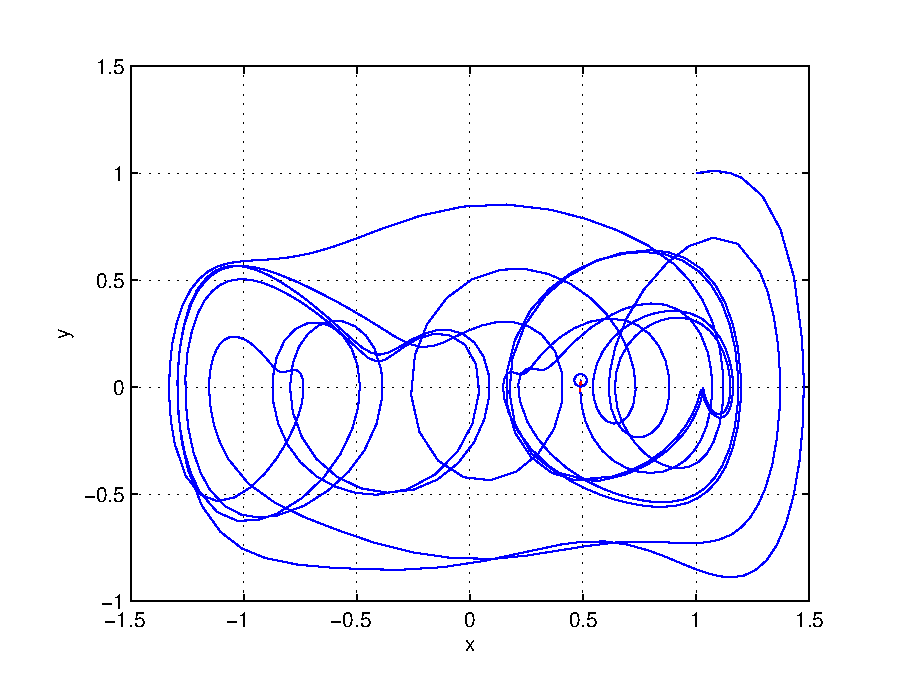
\includegraphics[width=1\linewidth]{duffing_chaos2.eps}}
	\caption{Фазовый портрет при ${\omega > \omega_{x}}$}
	\label{pic:duffing_chaos2}
\end{figure}
В качестве параметров уравнения применялись: $c = 0.5$, $\gamma=\gamma_{x}=0.36$, ${\omega=1}$

Часто для вычисления характеристик хаотической динамики применяется показатель Ляпунова.
Он показывает в каком состоянии находится система. Если система находится
в стабильном состоянии линии фазовой траектории будут близко прилегать одна к другой, в противном
случае система находится в состоянии хаоса. Детектор с применением показателя Ляпунова
представлен на рисунке \ref{pic:chaos_lyapunov}.
\begin{figure}[H]
	\center\scalebox{0.7}{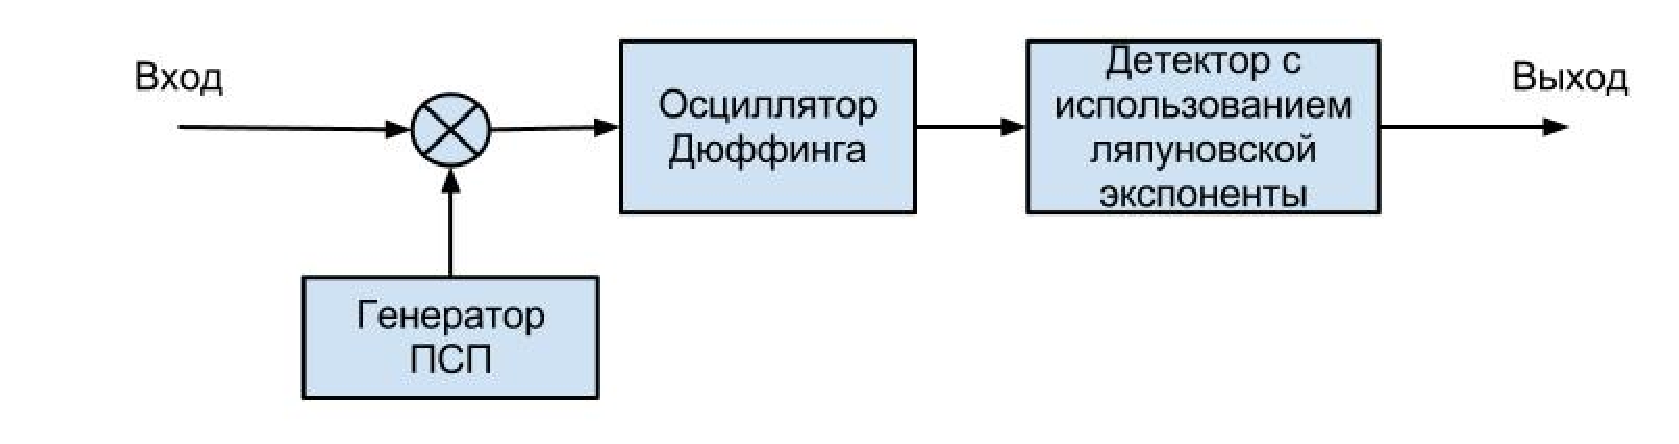
\includegraphics[width=1\linewidth]{Chaos_detector_Lyapunov.eps}}
	\caption{Схема детектора основанного на показателе ляпунова для осциллятора Дуффинга}
	\label{pic:chaos_lyapunov}
\end{figure}

В статье \cite{chaos_chen} предложен усовершенствованный метод, базирующийся на вычислении дисперсии
фазовой траектории. Действительно, на рисунках \ref{pic:duffing_sync}, \ref{pic:duffing_chaos1},
\ref{pic:duffing_chaos2} видно, что когда система находится в хаотическом состоянии значение
дисперсии по координате ${x}$ больше, чем соответствующее значение в состоянии $\omega = \omega_{x}$.
На основе этого была предложена усовершенствованная схема детектора сигнала - рисунок \ref{pic:chaos_energy_detector}
\begin{figure}[H]
	\center\scalebox{0.7}{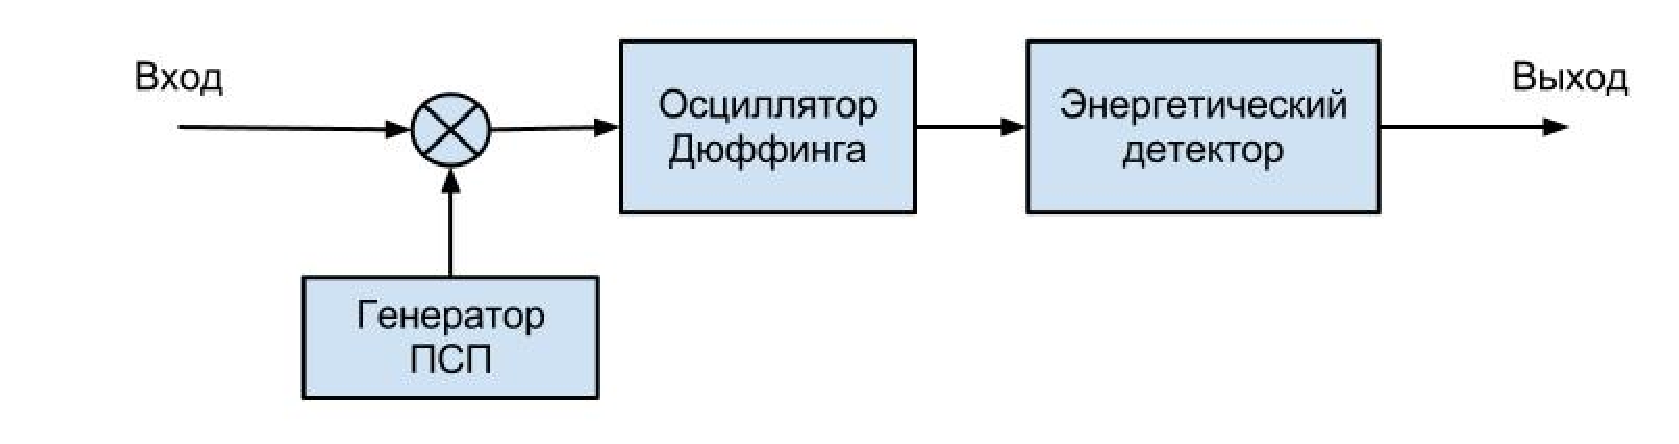
\includegraphics[width=1\linewidth]{chaos_detector.eps}}
	\caption{Схема энергетического детектора для осциллятора Дуффинга}
	\label{pic:chaos_energy_detector}
\end{figure}

%%%%%%%%
% HOS 
Математический аппарат статистик высоких порядков (СВП или HOS - Higher-order statistics)
для исследования непричинных, причинных и нестабильных (систем с неминимальной фазой) и негауссовых сигналов впервые был предложен
в \cite{hos_petropulu} в 1993 году.  Этот метод позволяет не только подавлять цветной Гауссов шум, но так же в некоторых случаях подавлять
цветной не-Гауссов шум.

В работе \cite{hos_zhao} был предложен метод детектирования ШПС с использованием СВП.

%%%%%%%%
% CHE 
Интересная группа алгоритмов основывается на информационной избыточности ШПС, например \cite{phd_che}. В данной
группе алгоритмов используется механизм появления нескольких точек на основном пике КФ, описанный в \cite{kaplan}. Пример
изображен на рисунке \ref{pic:sec1_peak_tcd}.
\begin{figure}[H]
        \center\scalebox{1}{\includegraphics[width=1\linewidth]{corr_peak_tcd.eps}}
        \caption{Идеальная КФ ШПС с отмеченными точками возможного обнаружения}
        \label{pic:sec1_peak_tcd}
\end{figure}
На рисунке \ref{pic:sec1_peak_tcd} изображен пик КФ с несколькими точками. Две точки находятся выше порога ${\Pi=0.5}$.
В работе \cite{phd_che} рассмотрено создание субоптимального обнаружителя на основе информационной избыточности ШПС.
Получена целевая функция системы и намечены дальнейшие пути развития данного направления.

%%%%%%%%
% 2MAX 
Так же одним из направлений исследований является разработка алгоритмов выбора порога без априорной информации о величине ОСШ. Например,
в работах \cite{2max_ieee, 2max_article} представлен алгоритм нахождения пика (АНП) КФ (Peak-finding algorithm).

Данный алгоритм можно разбить на несколько шагов:
\begin{itemize}
\item[Шаг 1] Подсчитать КФ, используя метод предложенный с использованием параллельного коррелятора. 
\item[Шаг 2] Найти главный пик КФ, найти второй пик КФ, найти среднее значение КФ.
\item[Шаг 3] Нормализовать полученные значения относительно главного пика КФ.
\item[Шаг 4] Если (максимум КФ - среднее) > ${\Pi_1}$ и (максимум КФ - 
	второй максимум КФ) > ${\Pi_2}$, тогда полученный главный пик КФ соответствует
	искомой фазе ПСП и частоте.
\end{itemize}

В статье авторов \cite{2max_ieee} предложены следующие значения для порогов:
${\Pi_1} = 0.3$ дБ и  ${\Pi_2} = 0.15$ дБ. Так же авторы предлагают итерационную процедуру для нахождения
фазы ПСП и частоты смещения допплера:
\begin{itemize}
\item[Шаг 1] Начать вычисление с 1мс.
\item[Шаг 2] Получить результаты АНП.
\item[Шаг 3] Если фаза ПСП и частота не могут быть найдены, увеличить время интегрирования сигнала.
	Использовать следующие значения для интегрирования: 1мс -> 10мс -> 50мс -> 100мс -> 200мс ->
	500мс -> 1000мс
\end{itemize}

Очевидным минусом данного подхода является сильная зависимость от интерференции. В городском каньоне будет присутствовать
несколько достаточно мощных лучей, а значит разница в энергии первого и второго пика будет низкой.

%%%%%%
\paragraph{Выводы.}

Во введении кратко приведена история развития СПИ с ШПС, приведены ученые внесшие значительный вклад в разработку данного направления связи. Так же рассмотрена
актуальность исследования в данной области. Кроме того, приведены определения, что такое СПИ с ШПС, ее математическая модель и основные отличительный особенности данного класса систем.
Так же приведены классические и новые подходы к оценке параметров СПИ с ШПС. Рассмотрен оптимальный алгоритм - последовательный коррелятор,
а так же новые достаточно экзотические подходы - применение осциллятора Дуффинга. 

\newpage

\paragraph{В первой} главе рассмотрен алгоритм оценки параметров сигнала от одного источника в широкополосных системах связи на
фоне аддитивного гауссового  шума.

Схема алгоритма представлена на рисунке \ref{pic:ar_cdma1_scheme1}.

\begin{figure}[H]
	\center\scalebox{0.9}{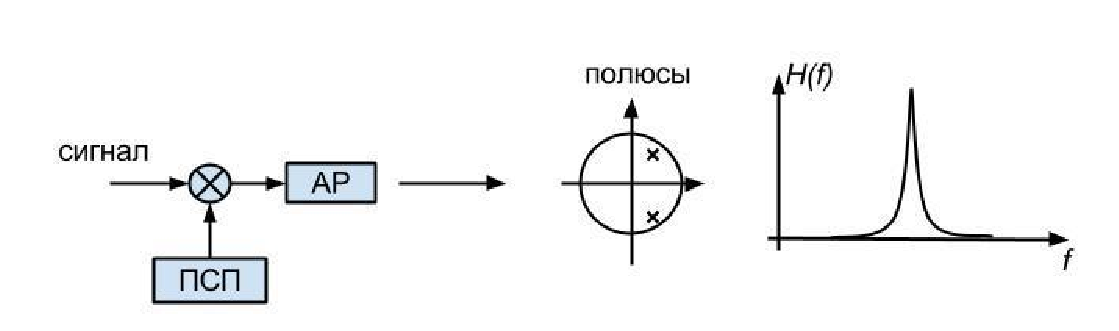
\includegraphics[width=1\linewidth]{lpc_for_1_sat_scheme.eps}}
	\caption{Детектирование сигнала АР-методом при известной фазе ПСП.}
	\label{pic:ar_cdma1_scheme1}
\end{figure}

Для восстановления гармонического сигнала из ШПС входная последовательность умножается на локально сформированную ПСП.
Далее запускается алгоритм на основе АР-модели. В реальных условиях приемник не имеет информации о фазе ПСП поэтому для детектирования
сигнала необходимо перебрать все возможные смещения расширяющего кода. Для ускорения вычислений предлагается использование алгоритма
быстрого преобразования Фурье (БПФ).
Схема вычислений представлена на рисунке \ref{pic:ar_cdma1_scheme2}.

\begin{figure}[H]
	\center\scalebox{0.9}{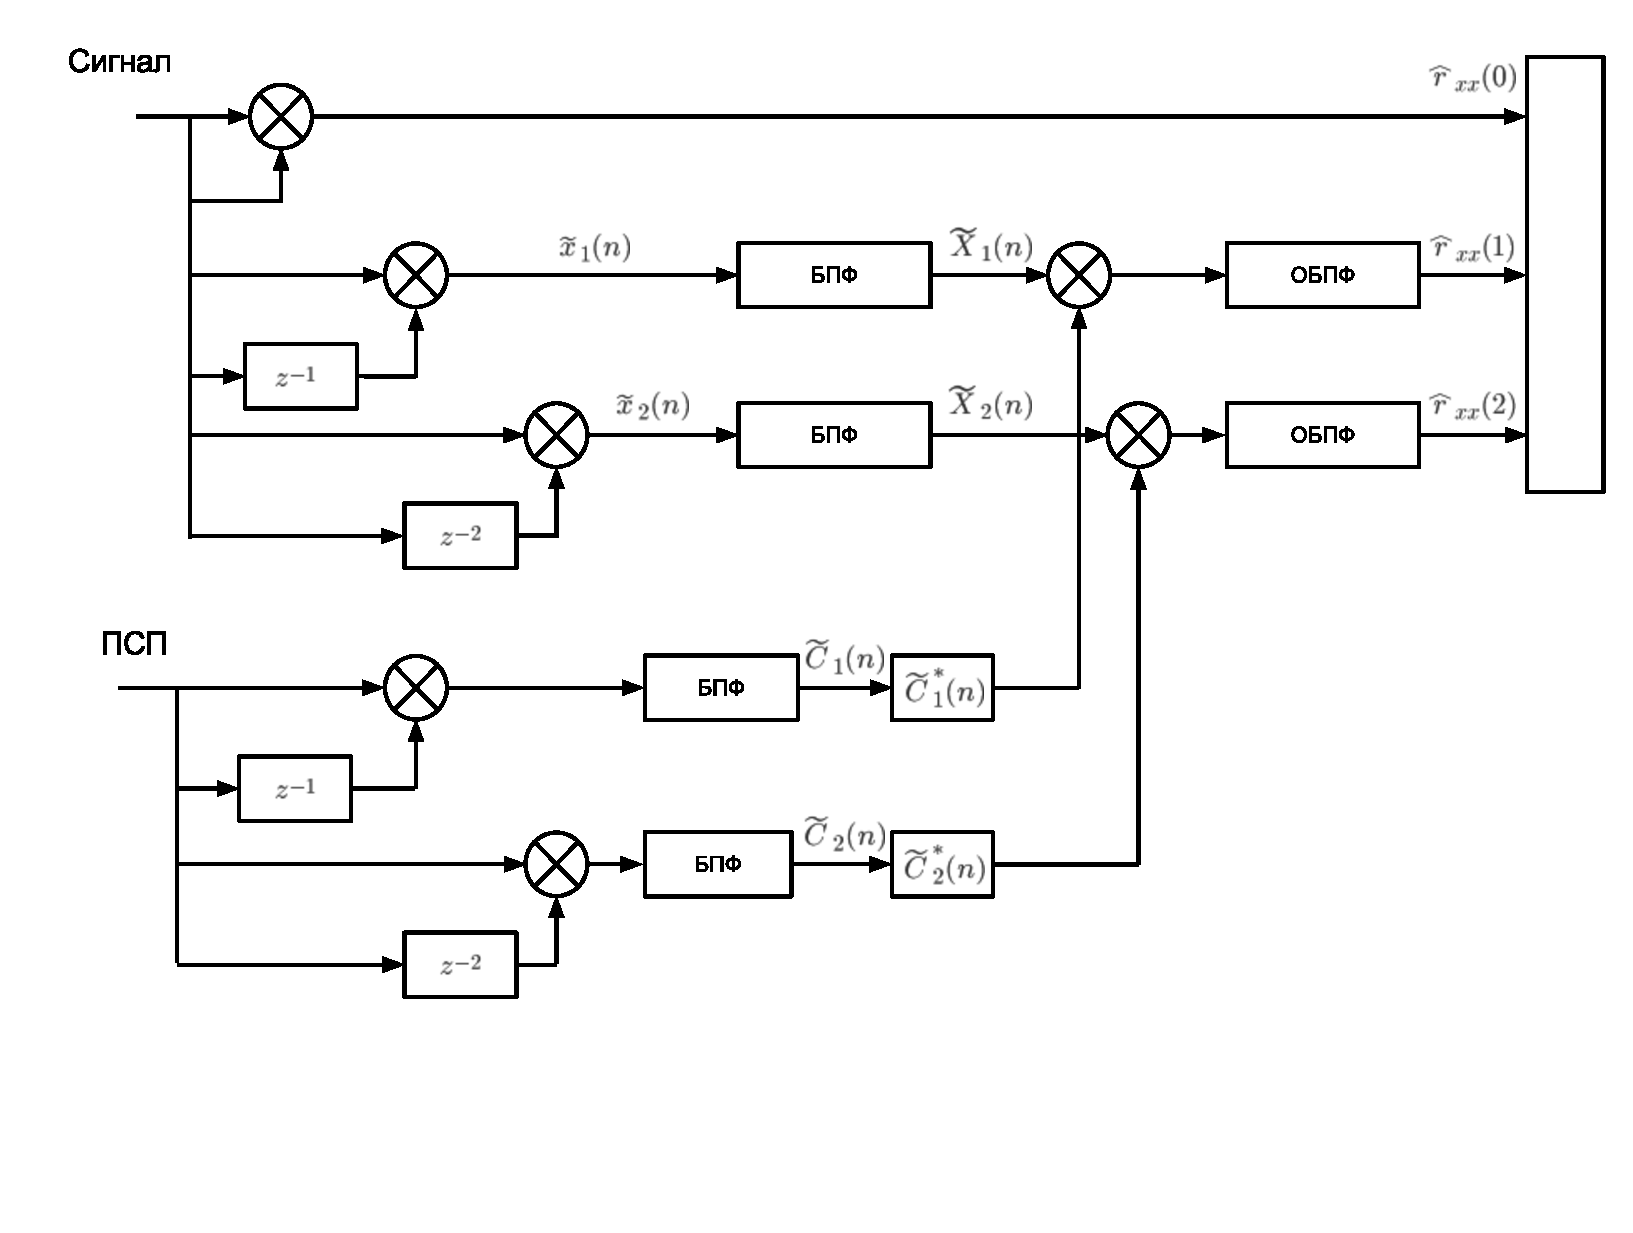
\includegraphics[width=1\linewidth]{lpc_fft.eps}}
	\caption{Общая схема применения АР модели для детектирования ШПС сигнала.}
	\label{pic:ar_cdma1_scheme2}
\end{figure}

Оценка ${\hat{r}_{xx}(0)}$ не зависит от выбранной фазы ПСП, поэтому она вычисляется один
раз для всех смещений кода. Далее формируется массив произведений входного сигнала на
свою задержанную копию ${\tilde{x}_1(n)=x(n)x(n-1)}$. Полученная последовательность  
${\tilde{x}_1(n)}$ поступает на вход алгоритма БПФ, в результате получаем массив ${\tilde{X}_1(n)}$
содержащий частотные отсчеты. Аналогично формируется массив  ${\tilde{X}_2(n)}$ для
задержки входного сигнала равной двум. Таким же способом обрабатываются локально
сгенерированные ПСП и формируются два массива ${\tilde{C}_1(n)}$ и ${\tilde{C}_2(n)}$.
Далее массивы ${\tilde{X}_1(n)}$ и ${\tilde{X}_1(n)}$ поэлементно перемножаются
на комплексно сопряженные массивы ${\tilde{C}_1^*(n)}$ и ${\tilde{C}_2^*(n)}$.
Результаты этих перемножений поступают на вход алгоритма обратного
БПФ. Полученные после ОБПФ два массива содержат оценки автокорреляционной функции для ${N}$ 
смещений кода, где  ${N}$ - размер данных на входе алгоритма БПФ.

Таким образом, предлагаемый алгоритм состоит из следующих шагов:

\begin{itemize}
\item[Шаг 1.] Вычисляются оценки  АКФ в трех первых точках (для аргументов АКФ=0,1,2)
	с использованием алгоритма БПФ для всех возможных смещений ПСП. 
\item[Шаг 2.] Для каждого смещения ПСП: 
	Определяются коэффициенты АР-модели ${\hat{a_1}, \hat{a_2}}$,
	вычисляется резонансная частота ${\omega_0}$
	и определяется квадрат модуля частотного отклика АР-модели для этой частоты. 
\item[Шаг 3.] Выбирается смещение ПСП для которого значение квадрата модуля частотного отклика было максимальным. Полученное значение сравнивается с заранее выбранным порогом детектора. 
	\subitem{\underline{Если}}  значение оказалось больше порогового {\underline{то}} 
		принимается решение о наличии сигнала, а в качестве оценки
		частоты принимается значение ${\omega_0}$ соответствующее выбранному смещению ПСП. 
	\subitem{\underline{Иначе}} 
		Принимается решение об отсутствии гармонического сигнала.
\end{itemize}

Разработанный алгоритм позволяет производить оценку частоты гармонического сигнала без использования прямого перебора как это делается в большинстве современных алгоритмов.
Например, алгоритм Delay and Multiply Approach (DMA) позволяет производить поиск только по смещению ПСП,
но он не дает возможности прямой оценки частоты. 
Предложенный алгоритм допускает сокращение количества операций умножения при переборе значений фазы ПСП за счет использования алгоритма БПФ.

Основным недостатком предложенного алгоритма является сильная чувствительность по отношению к интерференционным помехам: наличие «окрашенного» шума приводит к
значительному смещению получаемых оценок частоты и мощности гармонического сигнала.

Количество операций для оценки параметров от одного источника на фоне АБГШ:
\begin{center}
\begin{equation}
	%\label{}
	OP_{AR\_FOR\_1} = 24NlogN + 63N
\end{equation}
\end{center}

График вероятности оценки частоты в допустимом диапазоне входной расстройки представлен на рисунке
\ref{pic:lpc_for_1_probability}. Моделирование проводилось с аддитивным шумом, заданным в полосе от 0 Гц до
половины частоты дискретизации для одного, двух и трех шагов уточнения АКФ. В данном случае значение частоты дискретизации равно 16.368 МГц.
\begin{figure}[H]
\center\scalebox{1}{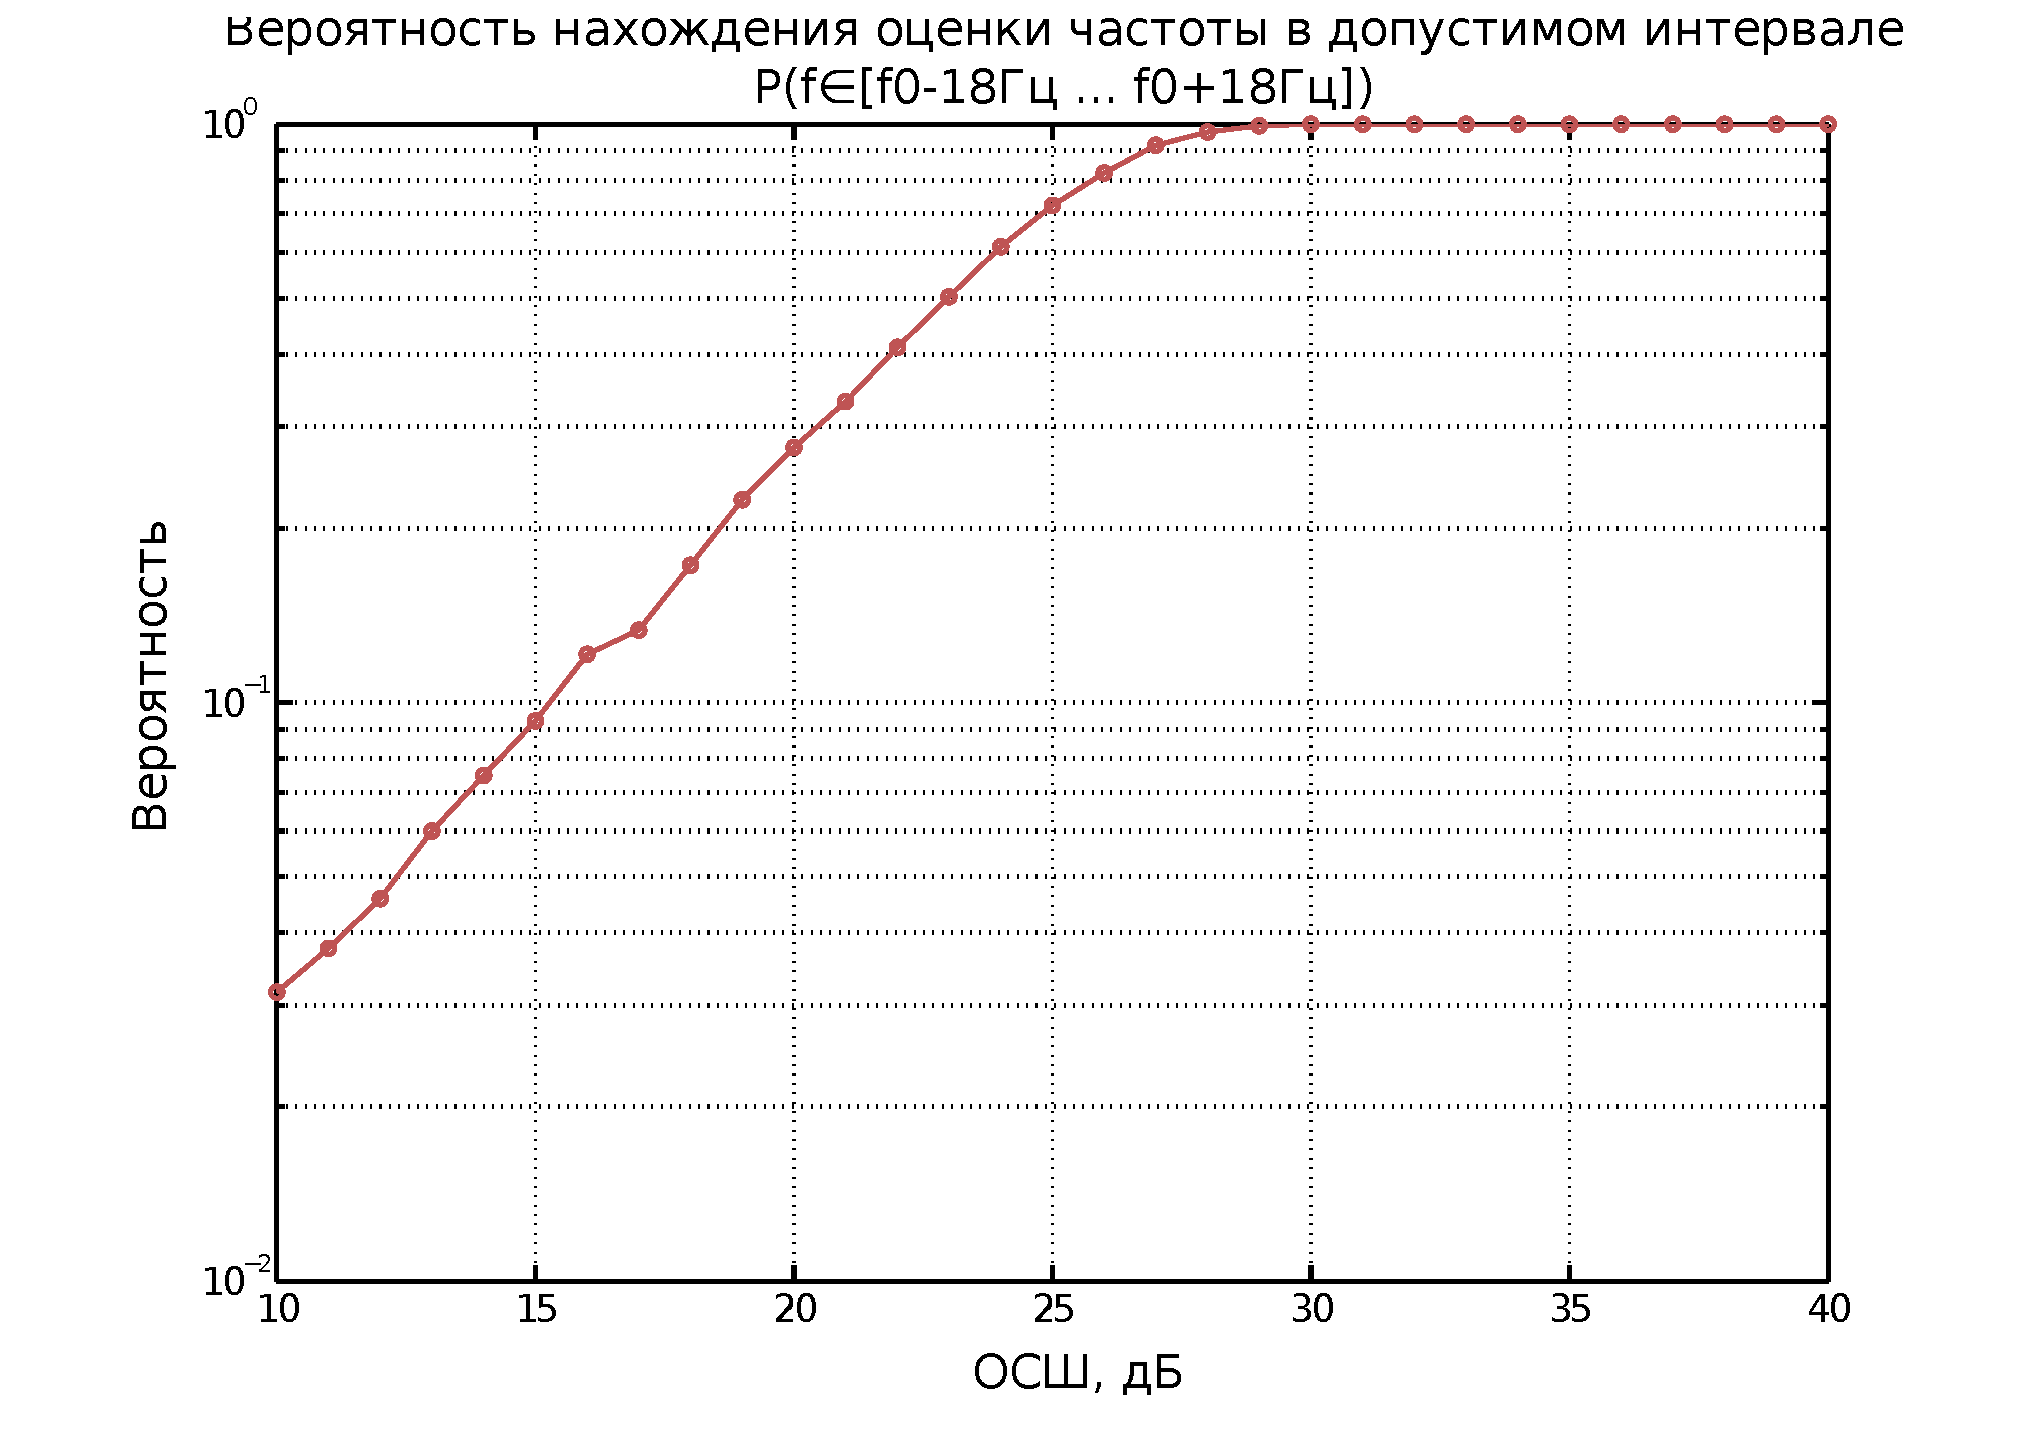
\includegraphics[width=1\linewidth]{lpc_for_1_probability.eps}}
	\caption{Вероятность оценки частоты удовлетворяющей допустимой входной расстройке}
	\label{pic:lpc_for_1_probability}
\end{figure}

Для оценки точности можно сравнить предлагаемый алгоритм с границей Крамера-Рао. Неравенство Крамера-Рао дает базу оценки, так
как представляет минимальную дисперсию оцениваемой величины среди всех классов оценщиков.
\begin{figure}[H]
\center\scalebox{1}{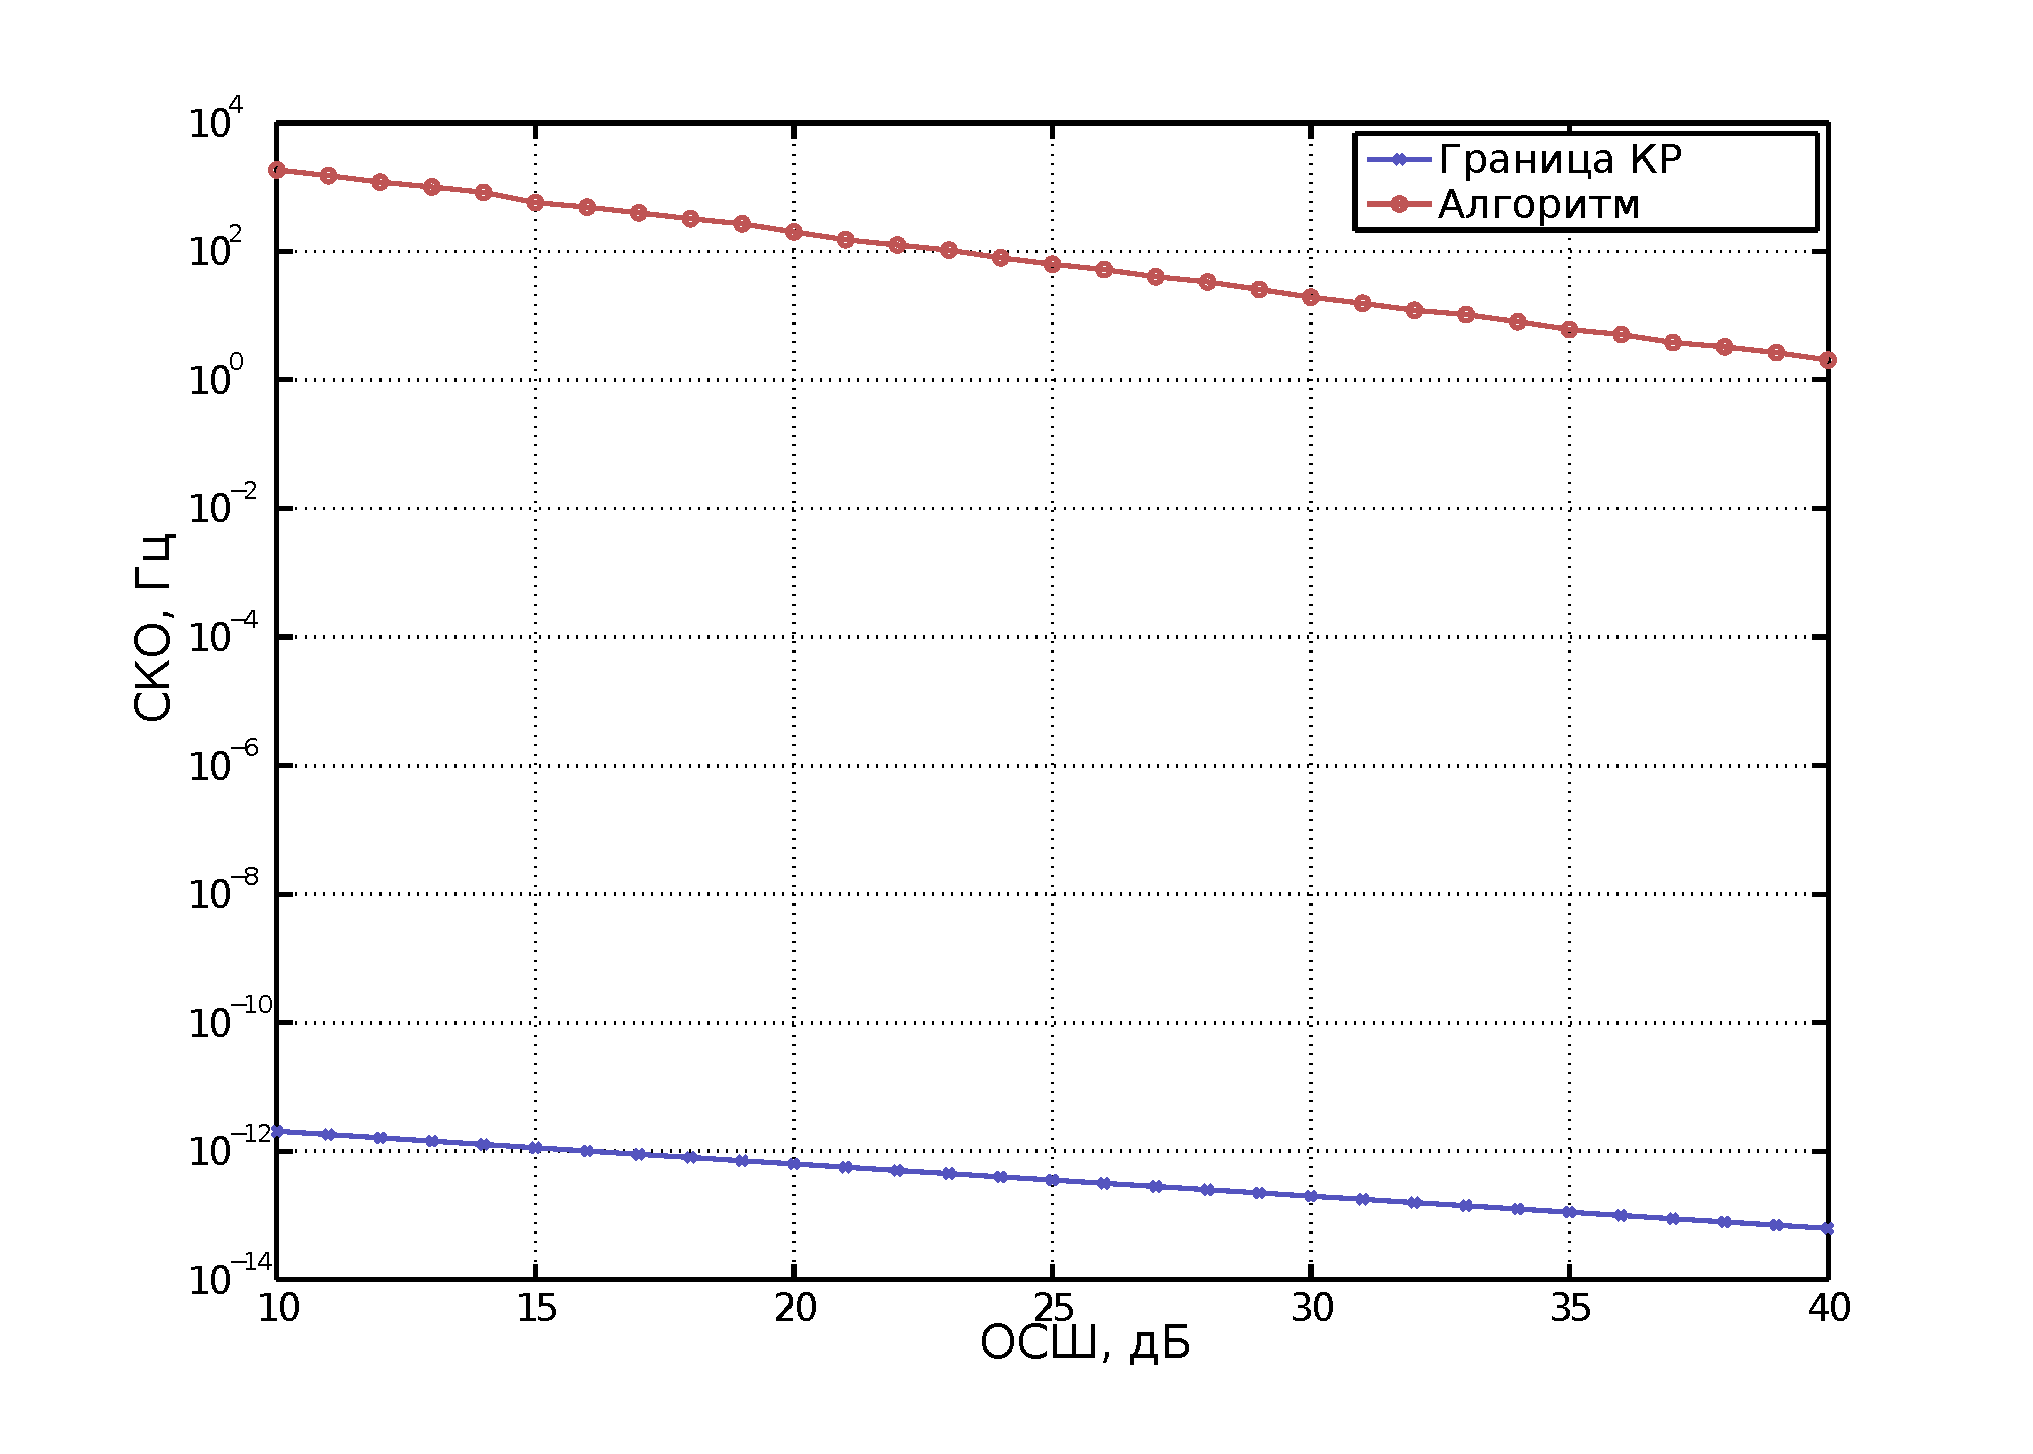
\includegraphics[width=1\linewidth]{crlb_vs_1sat_algo.eps}}
	\caption{СКО ошибка оценки частоты и граница Крамера-Рао в задаче оценки частоты гармонического сигнала}
	\label{pic:crlb_vs_1sat_algo}
\end{figure}

{\bf{Во второй}} главе выполнен синтез усовершенствованного алгоритма оценки автокореляционной функции (АКФ) с использованием
быстрого преобразования Фурье. Для верификации синтезированного алгоритма проведено имитационное моделироване.

Точность АР метода напрямую зависит от точности оценки АКФ гармонического сигнала.
Существует несколько способов компенсации шума для АР анализа.
Основным способом повышения точности оценки АКФ является увеличение размера выборки, что в случае фазомодулированного (ФМ) сигнала может быть затруднительным. 

В данной работе предлагается использовать алгоритм увеличения ОСШ методом итеративного вычисления АКФ.
Для снижения вычислительных затрат итеративное вычисление АКФ предлагается реализовывать в базисе Фурье. 

Уточненная оценка АКФ на ${K}$-ом шаге данного алгоритма может быть получена с помощью выражения:
\begin{center}
\begin{equation}
	\label{eq:akf_3}
	\hat{r}_K = F^{-1}\left[ \left| Fx \right| ^{2^K} \right],
\end{equation}
\end{center}
где ${x}$ – вектор входного сигнала после снятия ПСП, ${F}$ – матрица прямого преобразования Фурье,
${F^{-1}}$ - матрица обратного преобразования Фурье.

Схематически алгоритм получения уточненной оценки АКФ на третьем шаге представлен на Рис \ref{pic:akf_pic}.
\begin{figure}[h]
	\center\scalebox{1}{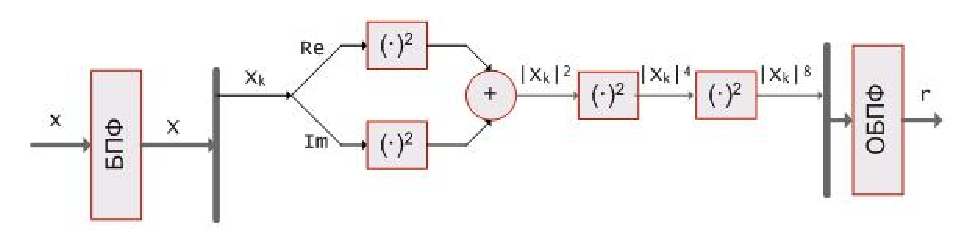
\includegraphics[width=1\linewidth]{akf_fft.eps}}
	\caption{Усовершенствованный итеративный алгоритм получения АКФ}
	\label{pic:akf_pic}
\end{figure}

Количество умножений необходимых для оценки АКФ при помощи прямого метода:
\begin{center}
\begin{equation}
	%\label{eq:}
	OP_{ACF} = 3N^2.
\end{equation}
\end{center}

Количество умножений необходимых для оценки усовершенствованным итеративным алгоритмом получения АКФ: \begin{center}
\begin{equation}
	%\label{eq:}
	OP_{ACF\_FFT} = 8NlogN + (k+2)N.
\end{equation}
\end{center}

%ОСШ в оценке АКФ по мощности можно вычислить по известной формуле:
%\begin{center}
%\begin{equation}
%	\label{eq:akf_max_eq}
%	R_s=2 B T R_e \frac{1}{2+1/R_e}
%\end{equation}
%\end{center}
%где ${R_s}$ - оценка ОСШ для АКФ, ${R_e}$ - ОСШ исходного сигнала, ${T}$ - длинна выборки (сек), ${B}$ -  ширина спектра сигнала.

%На рисунке \ref{pic:gps_spectrum} представлен спектр после повторной модуляции ПСП. 
% FIXME сделать сайд бай сайд до и после пересчета АКФ
В случае наличия интерференции, представляющей собой окрашенный шум, оценка параметрическим методом даст смещенное значение.
Применение усовершенствованного алгоритма итеративного вычисления АКФ позволяет получить ярко выраженный пик в спектральной области,
а СПМ приобретает симметричный вид, что позволяет использовать АР модель второго порядка для получения несмещенной оценки частоты
широкополосного сигнала.

После трех итераций предлагаемого алгоритма пик, соответствующий гармонической компоненте, существенно вырастает - Рис. \ref{pic:GPS_spectrum_iter3}.
\begin{figure}[h]
	\center\scalebox{1}{\includegraphics[width=1\linewidth]{GPS_spectra_iter3_new.eps}}
	\caption{Спектральная плотность мощности. а - входной смеси после повторной модуляции с ПСП, б - сигнала после 3 итерации уточнения АКФ}
	\label{pic:GPS_spectrum_iter3}
\end{figure}


\paragraph{В третьей} главе ставиться задача разработки алгоритма оценки информационных параметров CDMA-сигнала на основе алгоритма Delay and Multiply Approach,
предлагаемого усовершенствованного итеративного алгоритма вычисления АКФ и АР модели второго порядка.

В работе предлагается комплексировать результаты работы алгоритма Delay and Multiply Approach и, предложенных
в данной работе, усовершенствованного итеративного алгоритма уточнения АКФ гармонического
сигнала и подхода для оценки частоты CDMA-сигнала при помощи АР-модели.

При наличии нескольких источников CDMA-сигнала в смеси присутствует помеха в полосе сигнала.
После оцифровки и повторного модулирования входной смеси (\ref{eq:cdma_eq}) с ПСП в данном случае получается:
%
\begin{equation}
	\label{eq:cdma_strip_eq}
	x_k(m) = A_k \cos{(\tilde{\omega}_{k}m + \phi_k(m))} + n_k(m) + i(m)
\end{equation}
%
где ${m}$ - индекс соответствующий времени, ${\tilde{\omega}_k}$ - нормированная частота, соответствующая ${\omega_k}$, ${n_k}(m)$ - шум ${n(t)}$, умноженный на ПСП,
${i(m)}$ - интерференционная помеха.

Интерференционная составляющая ${i(m)}$ представляет собой сигнал от других источников, модулированный ПСП искомого источника сигнала:
\begin{equation}
	\label{eq:cdma_interference}
	i(m) = g_k(t) \sum\limits_{i=1, i \ne k}^{N}A_i g_i(t)\cos{(\omega_{i}m + \phi_i(m))}
\end{equation}

Схематично приемник изображен на Рис. \ref{pic:ar_dma_scheme}.
\begin{figure}[h]
\center\scalebox{1}{\includegraphics[width=1\linewidth]{dma_quadruple_lpc.eps}}
	\caption{Алгоритм оценки информационных параметров ШПС}
	\label{pic:ar_dma_scheme}
\end{figure}

Выходом алгоритма Delay and Multiply Approach является оценка фазы ПСП. Повторно модулируя входную смесь с ПСП,
можно восстановить гармонический сигнал при условии правильной оценки фазы ПСП. Для оценки частоты данного сигнала применяется
АР-метод. Но для оценки АР-методом, требуется точная оценка АКФ, которую можно получить
с помощью усовершенствованного итеративного алгоритма вычисления АКФ.

{\underline{Предложенный алгоритм можно описать следующим набором шагов:}}
\begin{itemize}[align=left,style=nextline,leftmargin=*,labelsep=\parindent,font=\normalfont]
\item[Шаг 1.] Входной сигнал ${x(m)}$ умножается на задержанную копию ${x(m-\tau)}$. Так же
	на данном шаге можно производить когерентное накопление результата, для
	увеличения ОСШ.
%
	\begin{equation}
		%\label{}
		x_{new}(m) = \frac{g_{new}(k)}{2} \left(\cos (2\pi f \tau) - \cos \left[2 \pi f (2m - \tau)\right]\right)
	\end{equation}
%
\item[Шаг 2.] Полученный сигнал ${x_{new}(m)}$ фильтруется ФНЧ для отсечения высокочастотной компоненты.
\item[Шаг 3.] Генерируется локальная ПСП ${C(m)}$ и умножается на задержанную копию ${g(m-\tau)}$.
%
	\begin{equation}
		%\label{}
		g_{new}(m) = g(m)g(m-\tau)
	\end{equation}
%
\item[Шаг 4.] Отфильтрованный сигнал ${x_{filt}(m)}$ коррелируется с новой ПСП ${g_{new}(m)}$
	с использованием БПФ. Выход коррелятора сравнивается с заранее определенным порогом.
%
	\begin{equation}
		%\label{}
		x_{filt}(m) = \frac{g_{new}(m)}{2} \cos (2\pi f \tau)
	\end{equation}
%
	\subitem{\underline{Если}}  значение оказалось больше порогового {\underline{то}},
		принимается решение о наличии сигнала. Полученное значение фазы ПСП  - ${k}$ запоминается.
		Перейти на шаг 5.
	\subitem{\underline{Иначе}} 
		Выбирается ${N}$ максимальных значений и запоминаются их фазы ПСП.
\item[Шаг 5.] Входная смесь ${x(m)}$ модулируется ПСП ${g(m-k)}$, где ${k}$ - это оценка фазы ПСП. В результате получаем гармонический
	сигнал ${x_{cos}(m)}$ с неизвестной частотой.
\item[Шаг 6.] Для увеличения ОСШ сигнала ${x_{cos}(m)}$ вычисляется значение уточненное значение АКФ
	по усовершенствованному итеративному алгоритму получения АКФ.
\item[Шаг 7.] Определяются коэффициенты АР-модели ${\hat{a_1}, \hat{a_2}}$.
	Вычисляется резонансная частота ${\omega_1}$ и определяется квадрат модуля частотного отклика АР-модели для этой частоты. 
\item[Шаг 8.]
	Сравнение квадрата модуля с порогом.
        \subitem{\underline{Если}}  значение оказалось больше порогового {\underline{то}} 
                принимается решение о наличии сигнала, а в качестве оценки
                частоты принимается значение ${\omega_1}$ соответствующее выбранной фазе ПСП. 
        \subitem{\underline{Иначе}} 
		\subsubitem\underline{Если} остались непроверенные фазы ПСП - переход на шаг 5.
		\subsubitem\underline{Иначе} сигнал не обнаружен.
\end{itemize}

График вероятности оценки частоты в допустимом диапазоне входной расстройки ФАПЧ для одной, двух и трех итераций уточнения АКФ представлен на Риc.
\ref{pic:ar_dma_probability}. Моделирование проводилось с аддитивным шумом, заданным в полосе от 0 Гц до
половины частоты дискретизации для одного, двух и трех шагов уточнения АКФ. В данной имитационной модели значение частоты дискретизации равно 16.368 МГц.
\begin{figure}[h]
\center\scalebox{1}{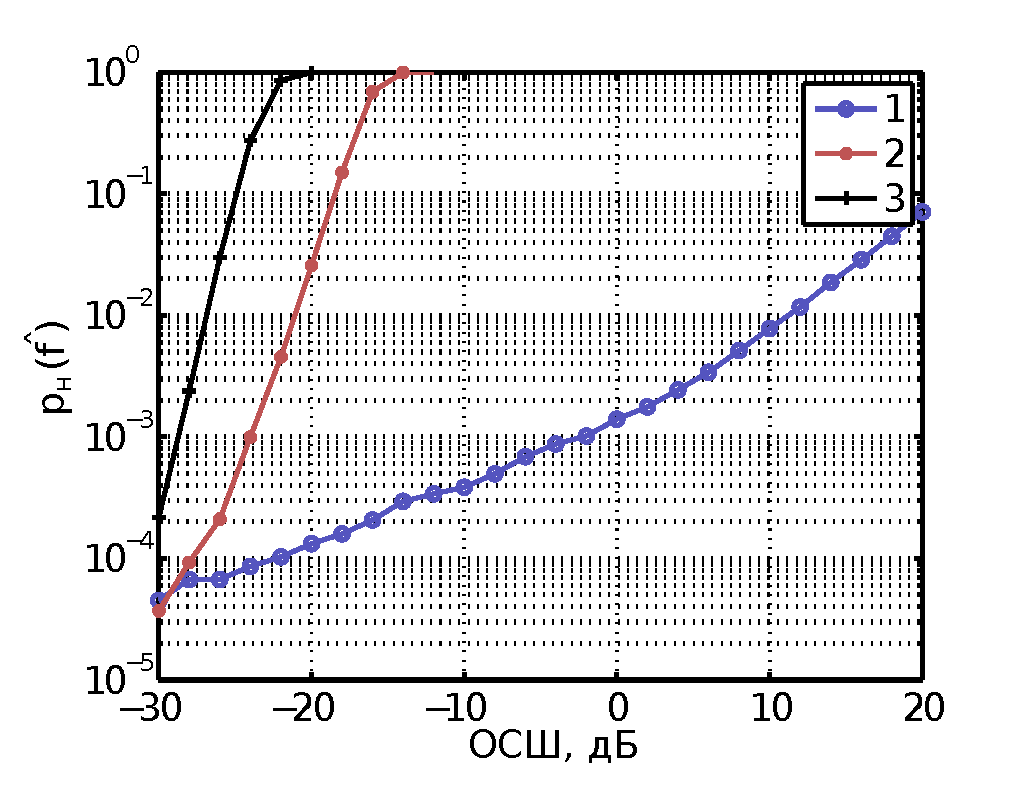
\includegraphics[width=1\linewidth]{ar_dma_probability.eps}}
	%\caption{Вероятность оценки частоты удовлетворяющей допустимой входной расстройке}
	\caption{ }
	\label{pic:ar_dma_probability}
\end{figure}

Так же в работе проводилось сравнение качества оценки частоты. График СКО ошибки при оценке частоты в зависимости
от ОСШ представлен на Рис. \ref{pic:crlb_vs_snr}. Для сравнения так же взята граница Крамера-Рао (КР).
\begin{figure}[h]
\center\scalebox{1}{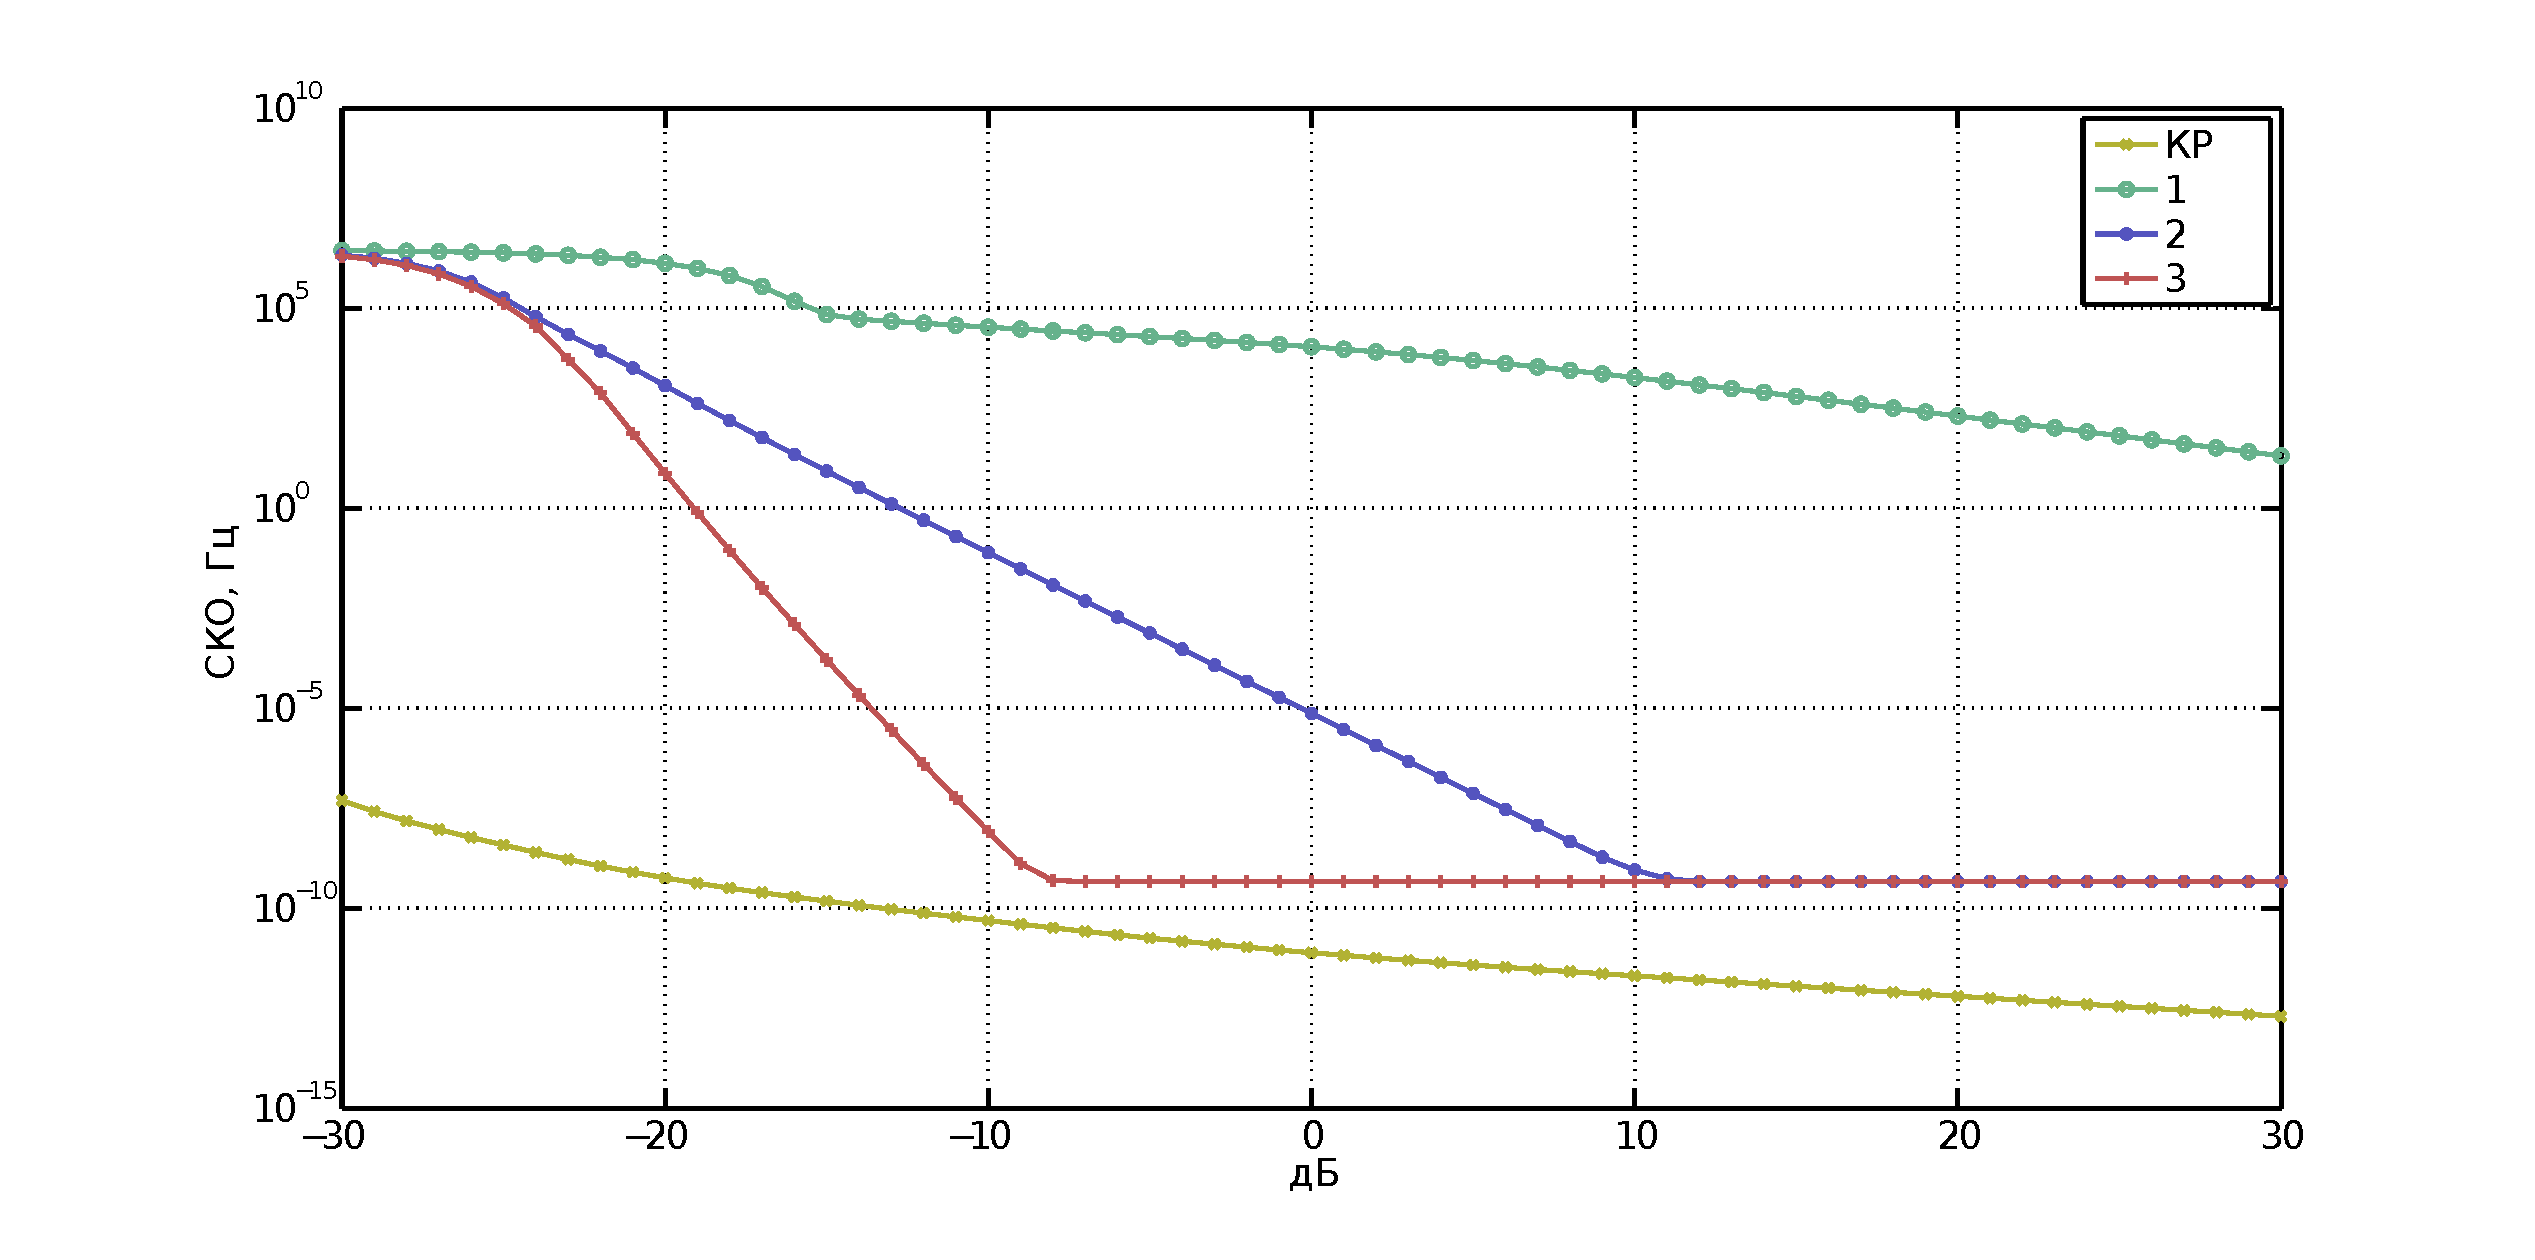
\includegraphics[width=1\linewidth]{crlb_vs_snr.eps}}
	%\caption{СКО ошибки оценки частоты и граница Крамера-Рао в задаче оценки частоты гармонического сигнала.}
	\caption{ }
	\label{pic:crlb_vs_snr}
\end{figure}

Единственным ограничением является наличие только одной гармонической компоненты в принимаемом сигнале.

Общее количество умножений, необходимых для оценки информационных параметров CDMA-сигнала от одного источника предлагаемым
алгоритмом (количество итераций в алгоритме уточнения АКФ равно 3): ${OP_{DMA\_ACF\_AR} = 16NlogN + 11N + 51}$.

Количество итераций требуемых для оценки частоты одного источника параллельным коррелятором:
${OP_{corr} = 48NlogN + 65N}$. Для оценки частоты берется входная последовательность равная 1 мс, что позволяет
получить точность 1 кГц, шаг одной итерации выбран в 1 кГц.

Предлагаемый подход существенно выигрывает по вычислительным затратам в сравнении с параллельным коррелятором при
меньших вычислительных затратах.

\paragraph{В четвертой} главе приводится полунатурный эксперимент по проверке рабочих характеристик предложенного комплексированного алгоритма
оценки информационных параметров CDMA-сигнала на фоне аддитивного белого гауссового шума и интерференционной помехи.
Эксперимент проводился на оригинальной, разработанной автором, программно-аппаратной платформе.
В качестве микросхемы захвата сигнала использовался чип от компании Maxim Semiconductor - MAX2769. Длинна записи, получаемой
с данной платформы для постобработки составляет 32 мс. Этого объема данных хватает для проверки качества работы алгоритма при оценке
параметров сигнала, но к сожалению не хватает для запуска модуля фазовой автоподстройки частоты для проверки вхождения в синхронизм и точной оценки частоты.

В данном случае, так как точное значение на выходе ФАПЧ получить не удается, за точное значение частоты бралось среднее значение математических
ожиданий всех оценок типового и комплексированного алгоритмов.

{\centering
\begin{longtable}{ | c | c | c |}
	\hline
	Алгоритм	& Вероятность	& Дисперсия, Гц \\
			& правильной оценки&		\\ \hline
	АР + DMA	& 0.52 & 16.13	\\ \hline
	Коррелятор 	& 0.80 &  21.56 \\ \hline
	\caption{Вероятность точной оценки предлагаемого комплексированного алгоритма и типового алгоритма с использованием этапа уточнения частоты}
	\label{tbl:16MHz}
\end{longtable}}

Так же в данной главе приводится полунатурное моделирование на данных, полученных из внешних источников. Длинна записи данных
позволяет оценить как параметры параметры сигнала, так и запустить модуль фазовой автоподстройки частоты для проверки вхождения в синхзронизм.

Результаты полунатурного эксперимента на данных, полученных из внешних источников, показали, что предлагаемый подход позволяет получить более точную оценку параметров
сигнала в системе с кодовым разделением каналов на примере системы Navstar GPS, а так же войти в синхронизм.

{\centering
\begin{longtable}{ | c | c | c | c |}
	\hline
	Алгоритм	& Вероятность	& Дисперсия, Гц & Среднее время \\
			& правильной оценки&		& вхождения в синхронизм\\ \hline
	АР + DMA	& 0.57 		& 15.42		& 21 мс \\ \hline
	Коррелятор 	& 0.84 		& 23.15 	& 34 мс \\ \hline
	\caption{Вероятность вхождения с синхронизм предлагаемого комплексированного алгоритма и типового алгоритма с использованием этапа уточнения частоты}
	\label{tbl:5MHz}
\end{longtable}}

Результаты данных полунатурных экспериментов показали, что предлагаемый подход позволяет получить более точную оценку параметров
сигнала в CDMA-системе на примере системы Navstar GPS.

%\paragraph{В четвертой} главе приводится имитационное моделирование развиваемых алгоритмов. В качестве алгоритма
%для сравнения используется параллельный коррелятор с алгоритмом уточнения частоты.
%
%\noindent{\begin{figure}[H]
%\center\scalebox{0.65}{\includegraphics[width=1\linewidth]{modeling_general.eps}}
%	\caption{Схема эксперимента}
%	%\label{pic:ar_dma_probability}
%\end{figure}}
%
%\underline{Алгоритм} оценки параметров сигнала с расширенным спектром на фоне аддитивного белого шума.
%График вероятности оценки частоты в допустимом диапазоне входной расстройки представлен на рисунке
%\ref{pic:lpc_for_1_probability}. Моделирование проводилось с аддитивным шумом, заданным в полосе от 0 Гц до
%половины частоты дискретизации для одного, двух и трех шагов уточнения АКФ. В данном случае значение частоты дискретизации равно 16.368 МГц.
%\begin{figure}[H]
%\center\scalebox{1}{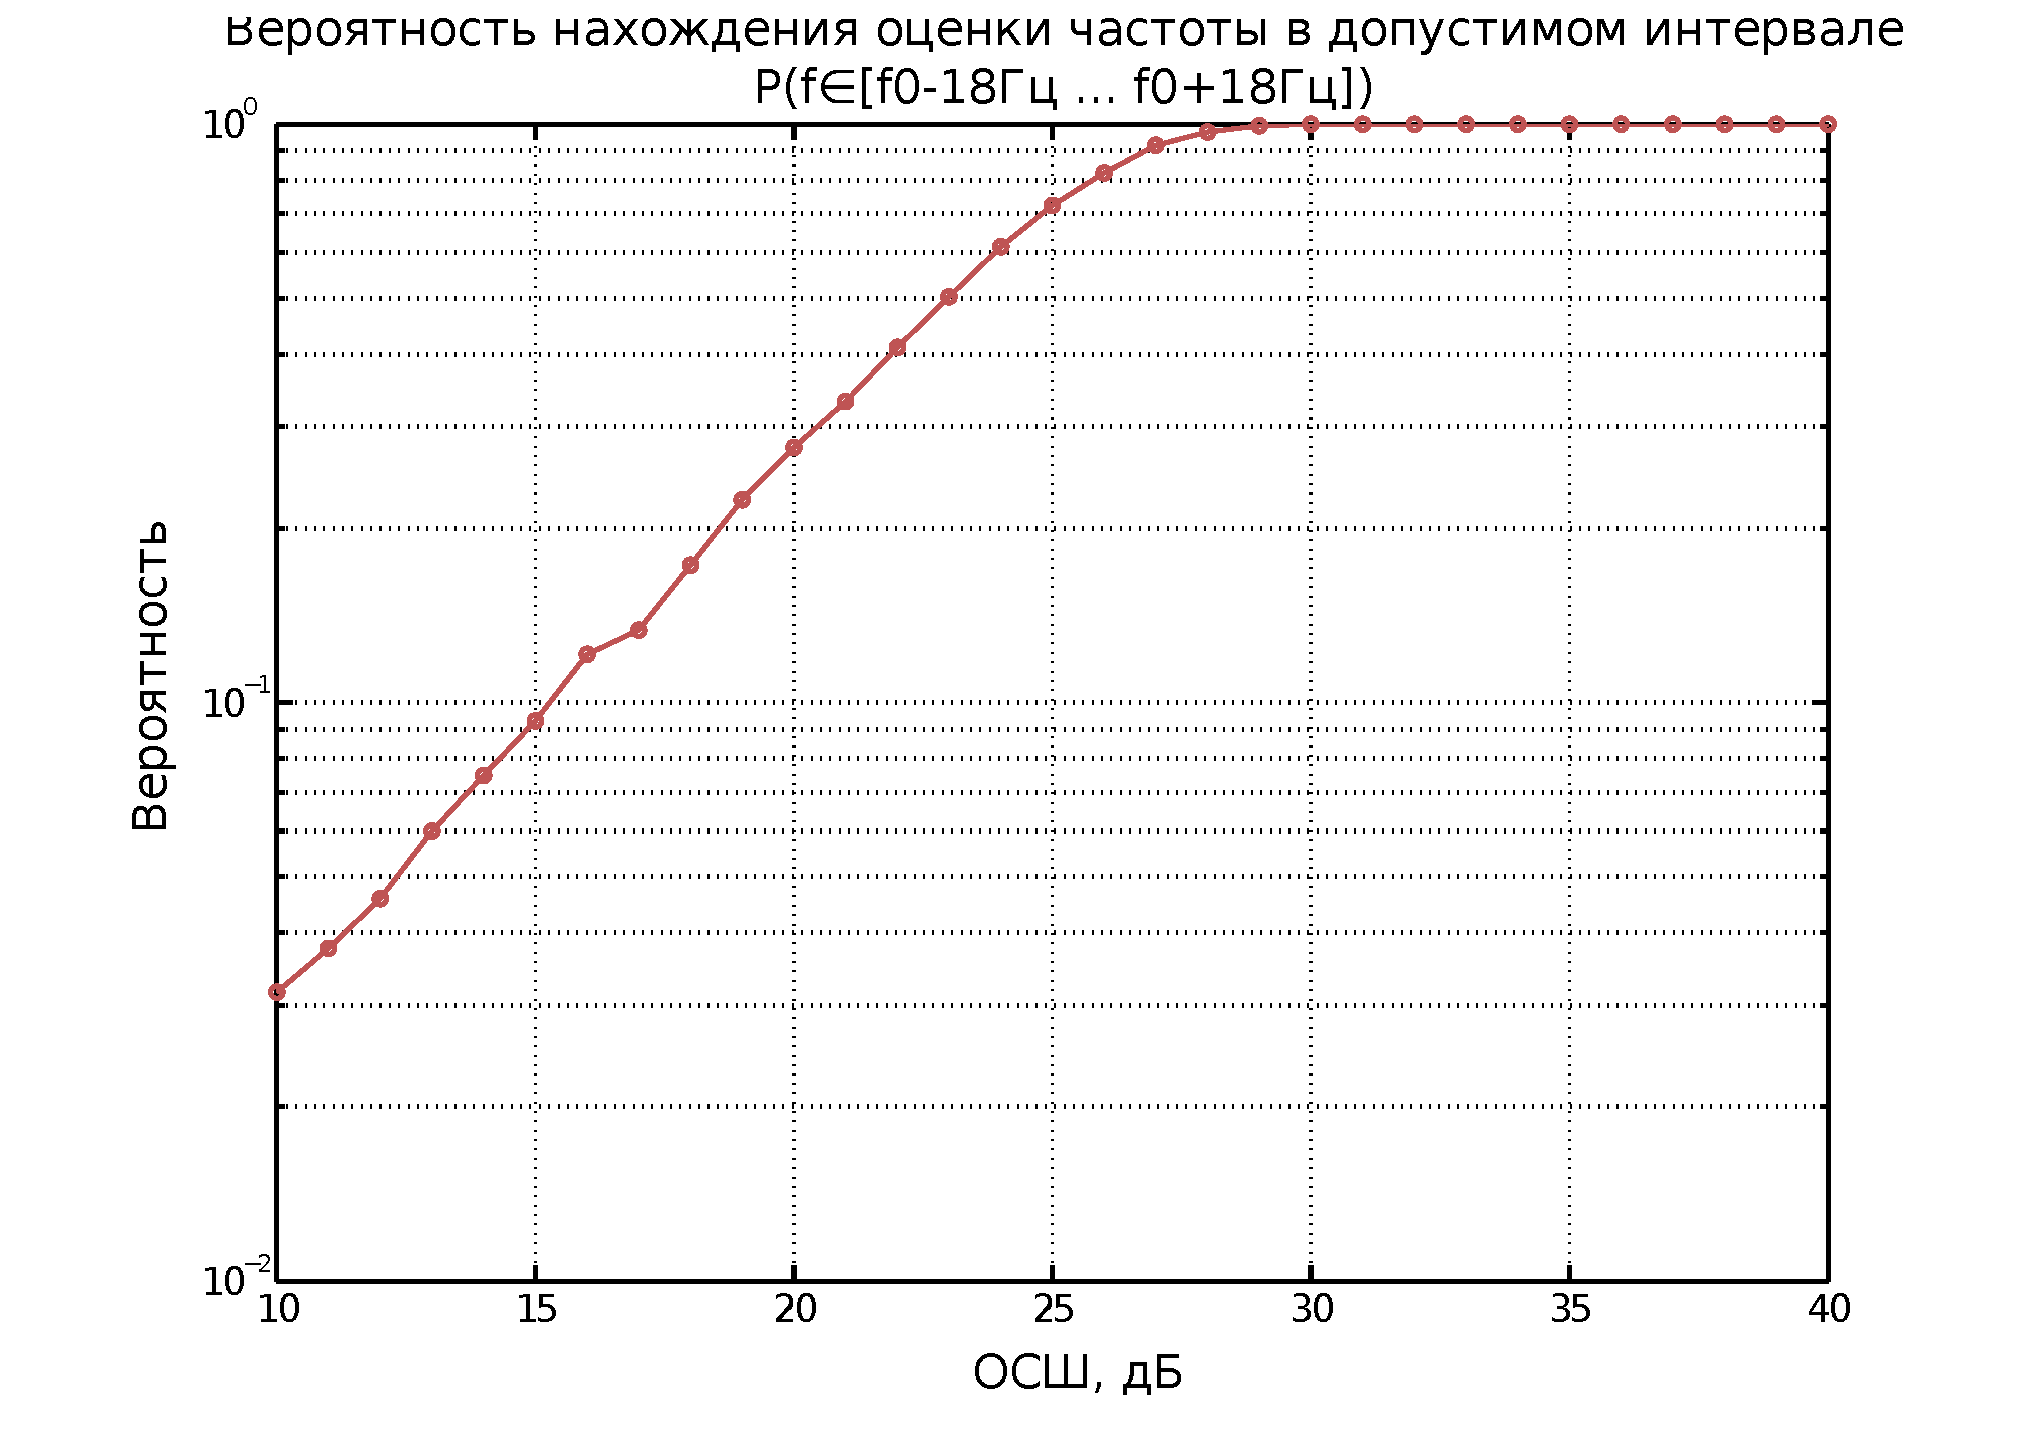
\includegraphics[width=1\linewidth]{lpc_for_1_probability.eps}}
%	\caption{Вероятность оценки частоты удовлетворяющей допустимой входной расстройке}
%	\label{pic:lpc_for_1_probability}
%\end{figure}
%
%Для оценки точности можно сравнить предлагаемый алгоритм с границей Крамера-Рао. Неравенство Крамера-Рао дает базу оценки, так
%как представляет минимальную дисперсию среди всех классов оценщиков.
%\begin{figure}[H]
%\center\scalebox{1}{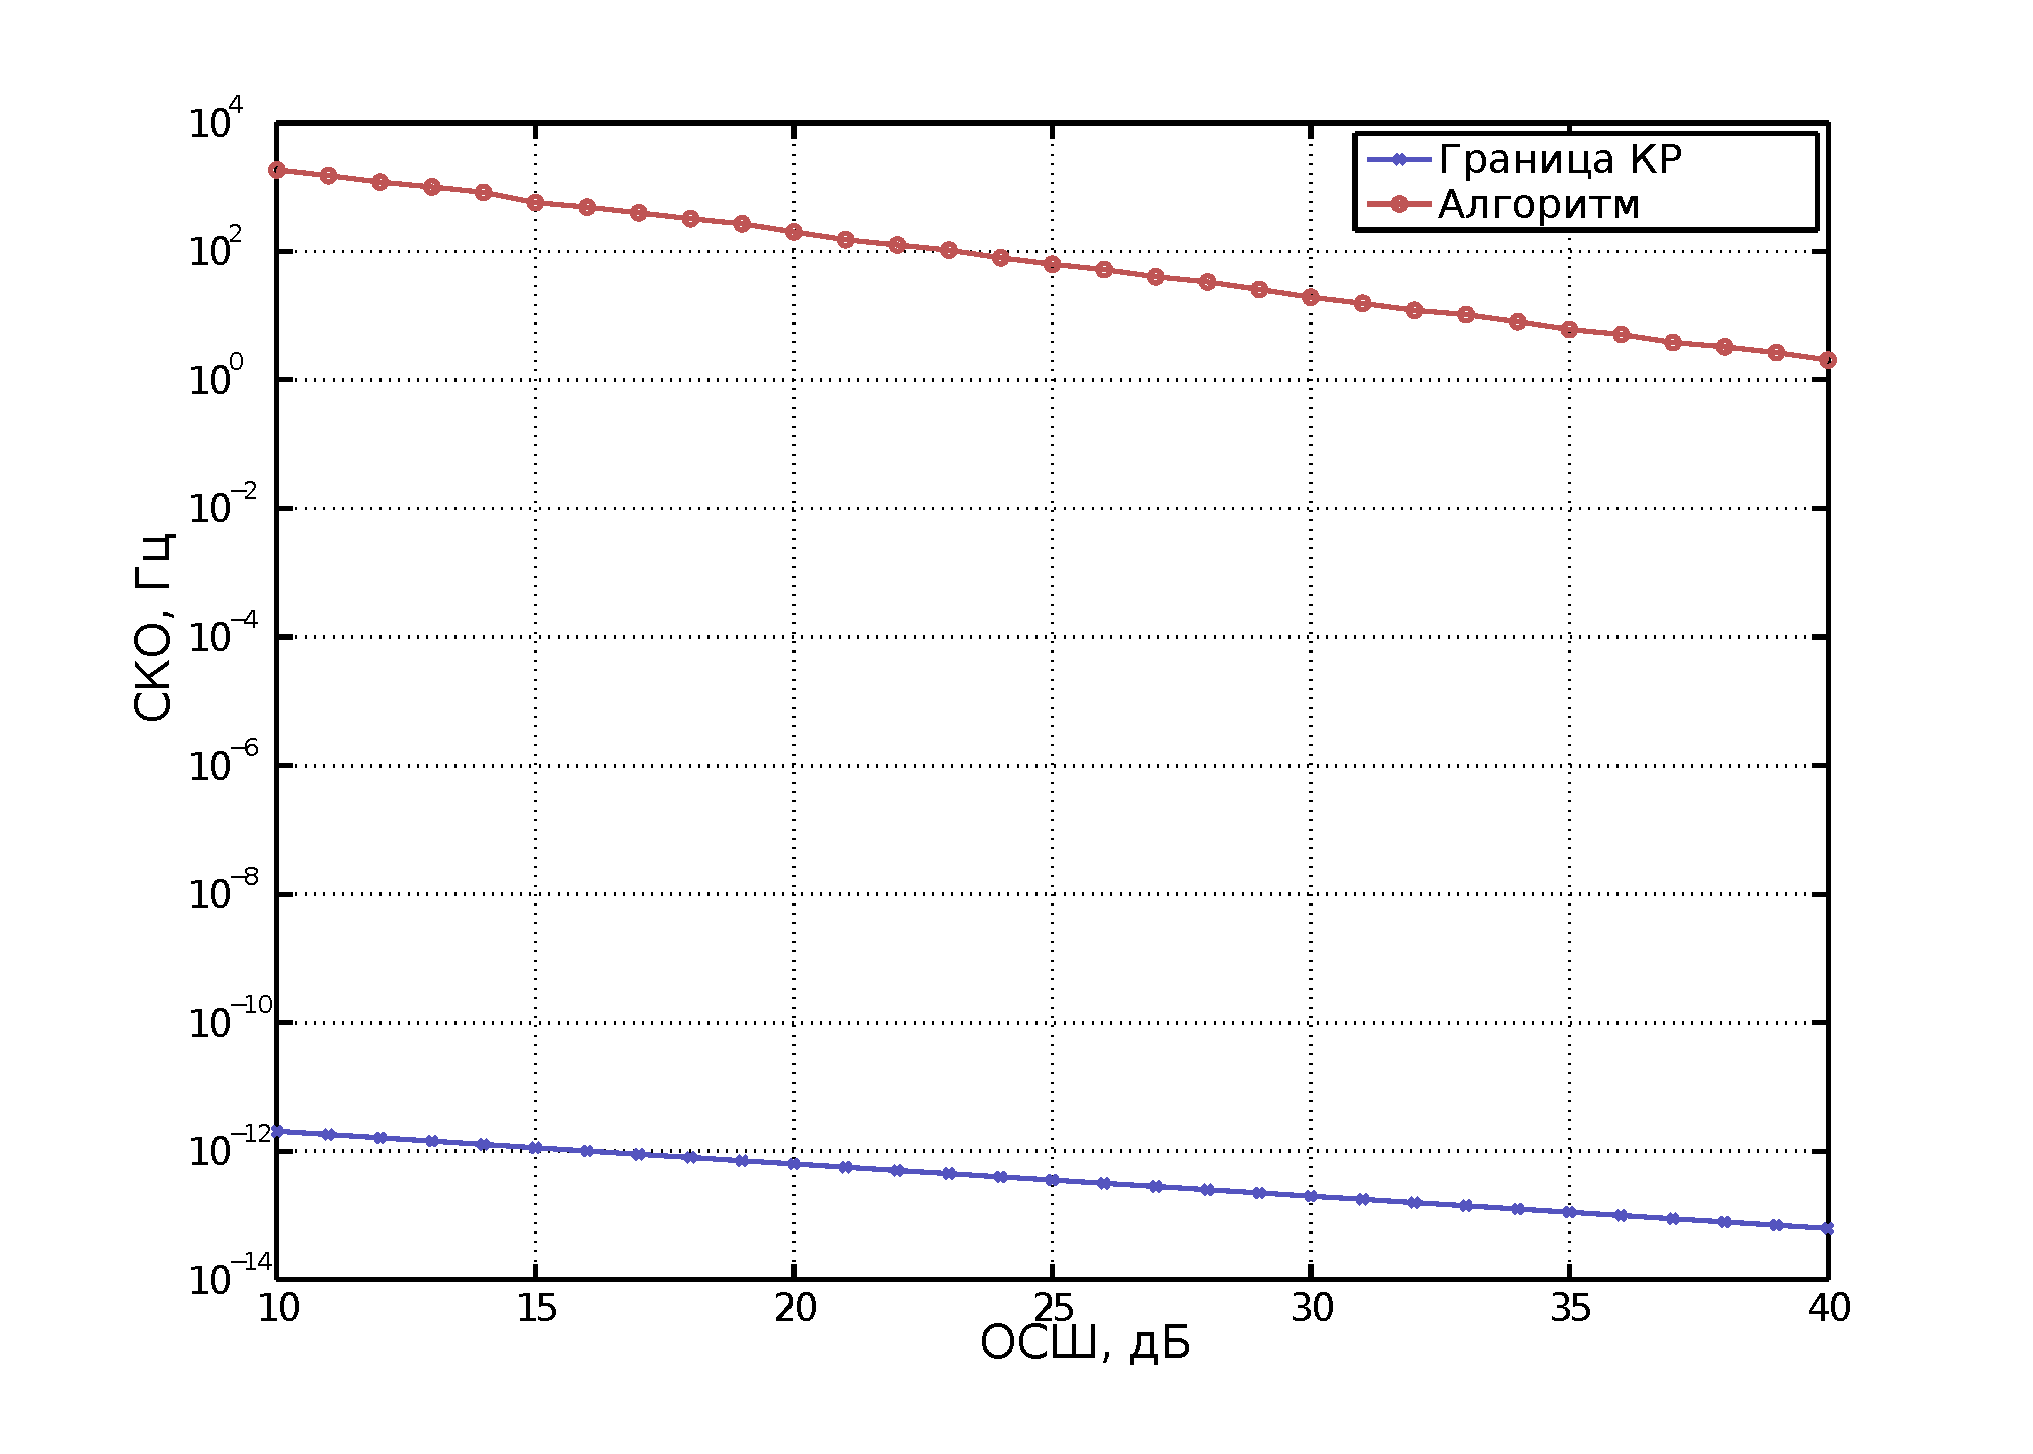
\includegraphics[width=1\linewidth]{crlb_vs_1sat_algo.eps}}
%	\caption{СКО ошибка оценки частоты и граница Крамера-Рао в задаче оценки частоты гармонического сигнала}
%	\label{pic:crlb_vs_1sat_algo}
%\end{figure}
%
%%%%%%%%%%
%\underline{Алгоритм} оценки параметров ШПС в условиях интерференции и аддитивного белого шума
%(Delay and Multiply Approach + уточненный АР).
%
%График вероятности оценки частоты в допустимом диапазоне входной расстройки представлен на рисунке
%\ref{pic:ar_dma_probability}. Моделирование проводилось с аддитивным шумом, заданным в полосе от 0 Гц до
%половины частоты дискретизации для одного, двух и трех шагов уточнения АКФ. В данной имитационной модели значение частоты дискретизации равно 16.368 МГц.
%\begin{figure}[H]
%\center\scalebox{1}{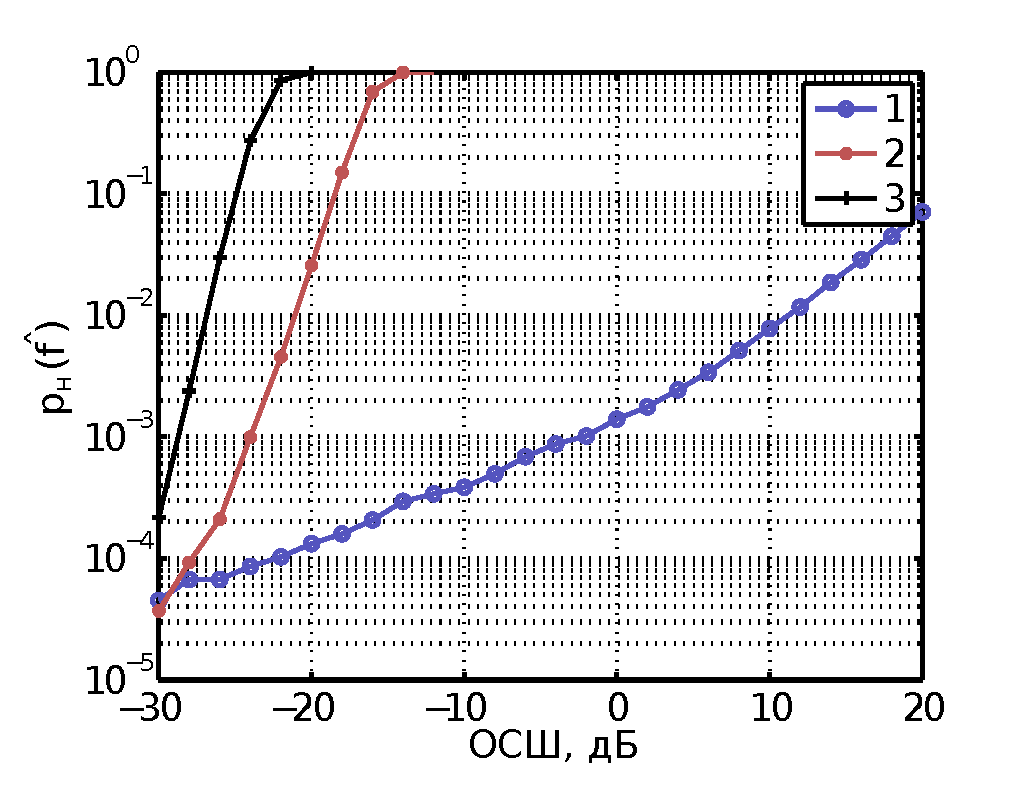
\includegraphics[width=1\linewidth]{ar_dma_probability.eps}}
%	\caption{Вероятность оценки частоты удовлетворяющей допустимой входной расстройке}
%	\label{pic:ar_dma_probability}
%\end{figure}
%
%Так же интересным является сравнение качество оценки частоты. График СКО ошибки при оценке частоты в зависимости
%от ОСШ представлен на рисунке \ref{pic:crlb_vs_snr}. Для сравнения так же взята граница Крамера-Рао (КР).
%\begin{figure}[H]
%\center\scalebox{1}{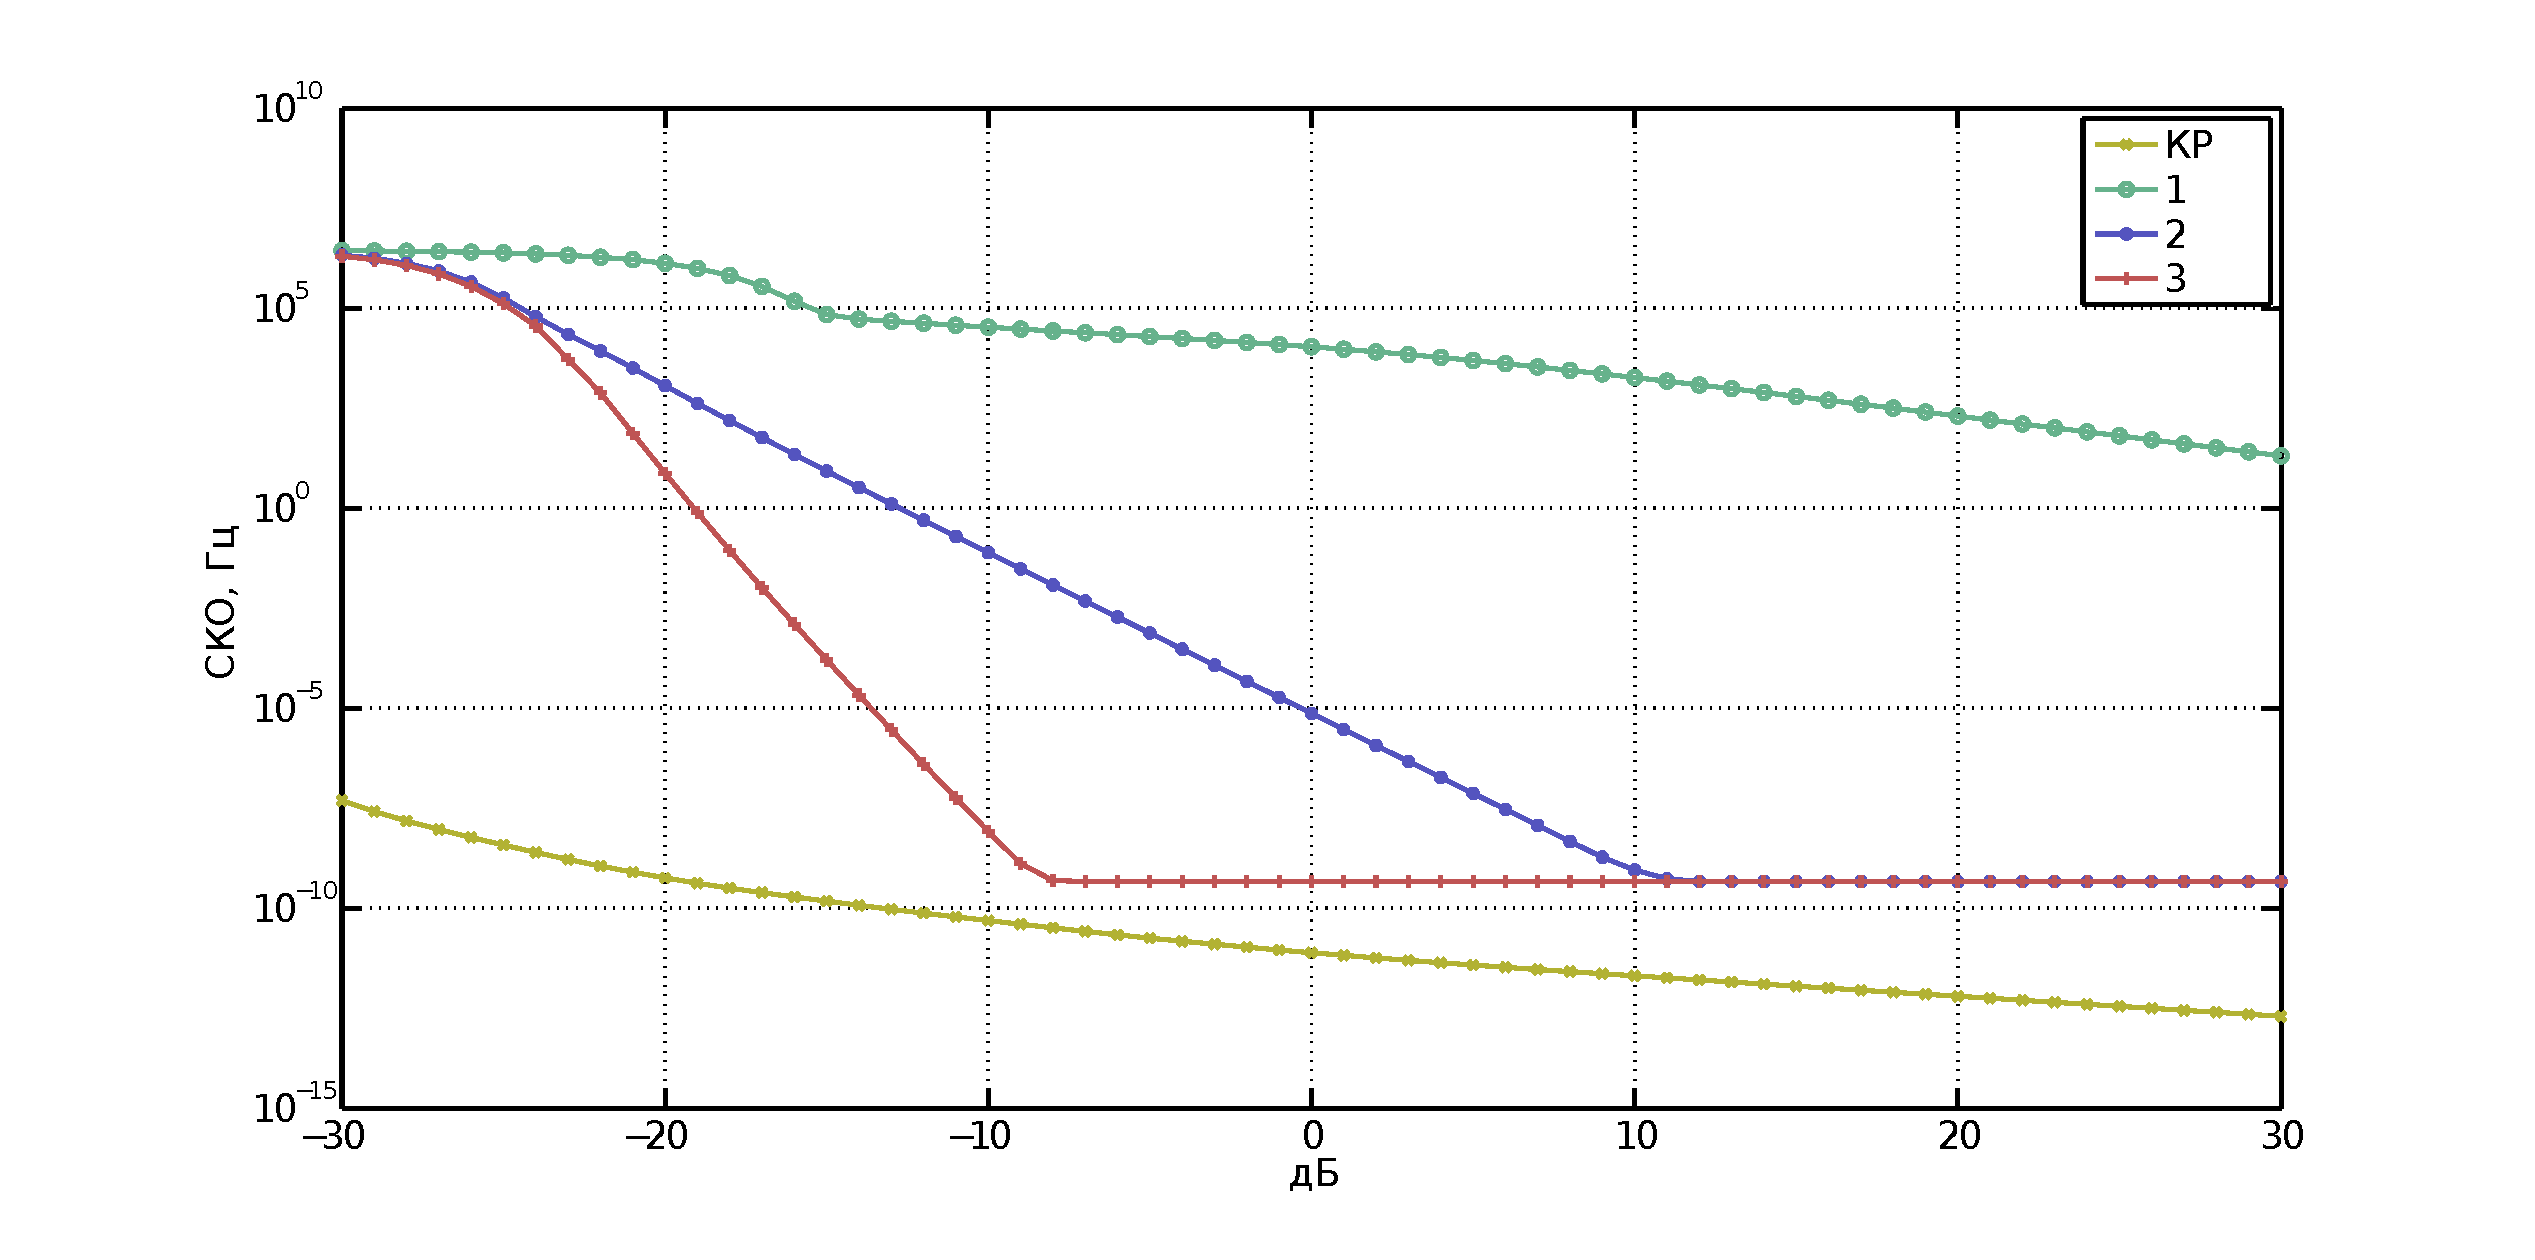
\includegraphics[width=1\linewidth]{crlb_vs_snr.eps}}
%	\caption{СКО ошибка оценки частоты и граница Крамера-Рао в задаче оценки частоты гармонического сигнала}
%	\label{pic:crlb_vs_snr}
%\end{figure}


{\bf{В заключении}}
отражены результаты работы и обозначены направления дальнейшего исследования

\noindent\centerline{\bf{Основные результаты и выводы}}
В ходе диссертационного исследования получены следующие результаты:
\begin{enumerate}
\item Разработан алгоритм на основе параметрического метода оценки частоты для одного источника с широкополосным сигналом.
\item Усовершенствован алгоритм итеративного вычисления автокорреляционной функции, что позволяет использовать его в приемниках
	реального времени.
\item Разработан алгоритм оценки параметров широкополосного сигнала на основе алгоритма Delay and Multiply Approach с использованием
	предложенного усовершенствованного итеративного алгоритма вычисления автокорреляционной функции и параметрического
	метода оценки частоты. Данное решение имеет более высокую точность оценки в сравнении с традиционным
	параллельным коррелятором, в то же время оценка параметра может быть получена за меньшее количество итераций.
\item Произведено имитационное моделирование предложенного алгоритма для проверки положений, выносимых на защиту.
\item Произведено обоснование актуальности и возможности применения параметрического метода оценки частоты для сигналов
	с расширенным спектром.
\item Отражены возможные направления дальнейших исследований в области применения параметрического анализа в системах
	с расширенным спектром.
\end{enumerate}


\newpage
